\documentclass[11pt]{article}
\usepackage[margin=1in]{geometry}
\usepackage{booktabs}
\usepackage{array}
\usepackage{longtable}
\usepackage{amsmath}
\usepackage{graphicx}
\usepackage{caption}
\usepackage{float}
\usepackage[table]{xcolor}
\usepackage{tikz}
\usetikzlibrary{arrows.meta,positioning,backgrounds,fit}
\usepackage[hidelinks]{hyperref}
\definecolor{vgreen}{HTML}{1B7837}
\definecolor{vorange}{HTML}{C97A0A}
\definecolor{vred}{HTML}{C0392B}
\definecolor{vgray}{HTML}{555555}
\definecolor{fd1c}{HTML}{1f77b4}
\definecolor{fd3c}{HTML}{C0392B}
\newcommand{\ttt}[1]{\texttt{#1}}
\newcommand{\verd}[2]{\textcolor{#1}{\textbf{#2}}}
\setlength{\parindent}{0pt}
\setlength{\parskip}{0.55em}


\begin{document}

\title{\textbf{The connectomic search for the FD4 figure-detection cell: a homogeneous \ttt{Nod1}/FD1 population and an honest null}}

\author{Stage 12 FD4 Identification}

\date{\today}

\maketitle

\tableofcontents

\part{Identity: the search for FD4 and its result}

\textbf{Summary.}\quad Egelhaaf defined FD4 as a progressive (front-to-back) figure-detection cell whose excitatory receptive field spans the whole horizontal extent of the ipsilateral eye and is most sensitive laterally, with no frontal gap, bidirectional contralateral inhibition, a cholinergic heterolateral noduli-group axon to the contralateral posterior optic foci, and a dendrite that spans the full horizontal but a restricted dorso-ventral extent of the lobula plate. This report searches the FlyWire connectome for that cell. The search returns a negative result. FD4 shares the entire output class of the already-identified FD1 cell (\ttt{Nod1}): progressive, heterolateral, cholinergic, and noduli-group. A funnel over all 8806 FlyWire cell types finds \ttt{Nod1} to be the sole progressive figure-output type; every other progressive midline-crossing cell is an inhibitory or centrifugal feedback element. The \ttt{Nod1} type contains four cells, but they form one homogeneous frontal population (no partition isolates a lateral, wide, dorso-ventrally restricted FD4 pair; homogeneous = True), most consistent with Egelhaaf's two anatomical FD1 variants, and none of them carries FD4's whole-eye lateral receptive field or restricted dorso-ventral dendrite. FD4 is therefore not individually resolved in FlyWire v783. The decomposed, null-aware confidence that FD4 is individually resolved is 0.0 (plausible range [0.0, 0.27]). The report states this negative result, its full evidentiary basis, and the complete progressive figure arm that any FD4 correlate would use.

\section{Introduction}

\textbf{Figure-ground discrimination and the FD cells.}\quad
A textured object is invisible against a matched background until it moves at a different velocity or
phase; relative motion then makes it salient. Reichardt and Poggio showed behaviourally that flies
detect and track such figures~\cite{rp1979}. Egelhaaf, in a three-part study, described a class of
lobula-plate tangential cells, the figure-detection (FD) cells, each more sensitive to a small moving
figure than to wide-field motion~\cite{egelhaaf1985b}. Four were distinguished by preferred direction
and receptive-field organisation. \textbf{FD1} is progressive with a narrow frontal field; \textbf{FD2}
is regressive with a frontal field; \textbf{FD3} is regressive with a fronto-lateral field and a
frontal gap; \textbf{FD4} is progressive with a receptive field that covers the whole horizontal
extent of the ipsilateral eye, is most sensitive laterally (peaks at azimuth $50$--$80^\circ$,
half-maximum width $80$--$110^\circ$, reaching beyond $120^\circ$), has no frontal gap, receives
bidirectional contralateral inhibition, and, like FD1 and FD3, is a heterolateral noduli-group output
element whose axon crosses to the contralateral posterior optic foci. Its dendrite spans the full
horizontal extent of the lobula plate but not its full dorso-ventral extent, and it has no second
arborisation in the lateral protocerebrum~\cite[p.~204--206]{egelhaaf1985b}.

\textbf{The connectome era and the mapping problem.}\quad
The adult \emph{Drosophila} FlyWire connectome and its cell-type annotations provide the
synapse-resolution wiring needed to ask which modern cell type corresponds to each FD
cell~\cite{dorkenwald2024,schlegel2024,codex}. T4 and T5 encode ON/OFF edge motion and segregate by
preferred direction into the four lobula-plate layers~\cite{maisak2013,fd1989}: layer-a front-to-back
(progressive), layer-b back-to-front (regressive). FD1 has been mapped to \ttt{Nod1}, FD2 to
\ttt{LPT21}, and FD3 to \ttt{LPT42\_Nod4}. This report asks which cell type is FD4.

\textbf{Why FD4 is the hard case.}\quad
The defining connectome signature of an FD output cell is its preferred direction (from its T4/T5
layer), its output side (from where its synapses land), and its transmitter. On all three, FD4 is
identical to FD1: both are progressive (layer-a), both are heterolateral (their axon crosses to the
contralateral posterior optic foci), and both are cholinergic. Egelhaaf states this directly: FD4
uses the same axonal pathway as the FD1nod and FD3 cells. FD4 is separated from FD1 only by its
receptive field (whole-eye and lateral, versus FD1's frontal and narrow) and by its dendrite (a
restricted dorso-ventral extent, versus FD1's full extent). The search for FD4 is therefore a search
for a progressive, heterolateral, cholinergic cell that is distinct from FD1 in receptive field and
dendrite. Figure~\ref{fig:concept} fixes the FD4 phenotype and the difficulty.

\begin{figure}[H]\centering
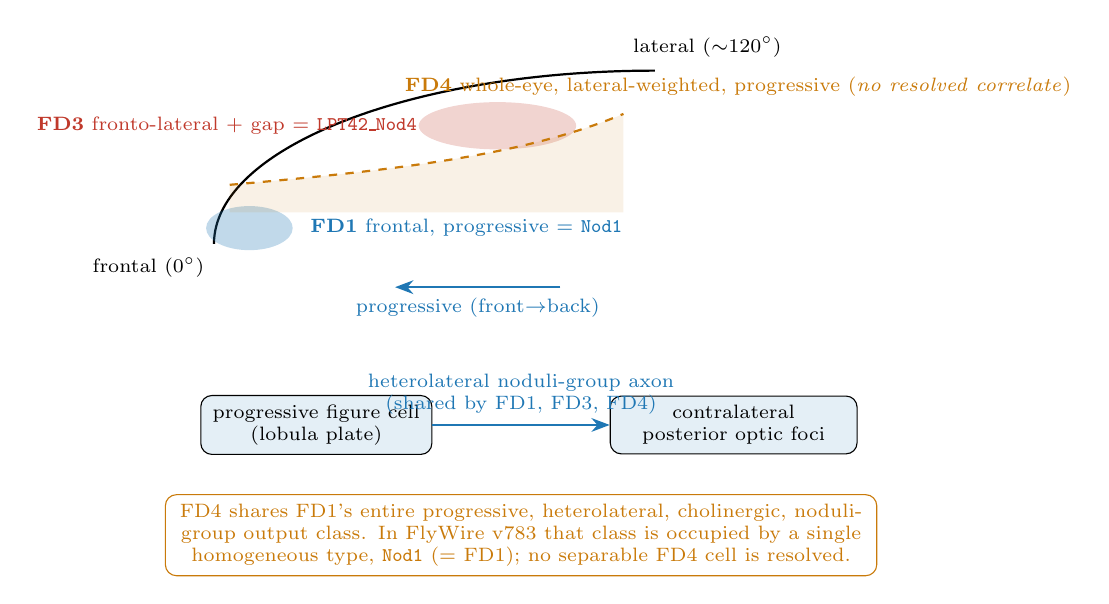
\begin{tikzpicture}[font=\small,>=Stealth]
  \draw[thick] (0,0) arc (180:90:5.6 and 2.2);
  \node[anchor=north east,font=\scriptsize] at (0,-0.05) {frontal ($0^\circ$)};
  \node[anchor=south west,font=\scriptsize] at (5.2,2.25) {lateral ($\sim$120$^\circ$)};
  % FD1 frontal (progressive)
  \fill[fd1c,opacity=0.28] (0.45,0.2) ellipse (0.55 and 0.28);
  \node[fd1c,font=\scriptsize,anchor=west] at (1.1,0.2) {\textbf{FD1} frontal, progressive $=$ \ttt{Nod1}};
  % FD3 fronto-lateral + gap (regressive)
  \fill[fd3c,opacity=0.22] (3.6,1.5) ellipse (1.0 and 0.30);
  \node[fd3c,font=\scriptsize,anchor=east] at (2.7,1.5) {\textbf{FD3} fronto-lateral $+$ gap $=$ \ttt{LPT42\_Nod4}};
  % FD4 whole-eye, lateral-weighted (dashed = not resolved)
  \draw[vorange,thick,dashed] (0.2,0.75) .. controls (2.5,0.95) and (4.0,1.15) .. (5.2,1.65);
  \fill[vorange,opacity=0.10] (0.2,0.75) .. controls (2.5,0.95) and (4.0,1.15) .. (5.2,1.65)
        -- (5.2,0.4) -- (0.2,0.4) -- cycle;
  \node[vorange,font=\scriptsize,anchor=west] at (2.3,2.0)
        {\textbf{FD4} whole-eye, lateral-weighted, progressive (\emph{no resolved correlate})};
  \draw[->,thick,fd1c] (4.4,-0.55) -- (2.3,-0.55)
        node[midway,below,font=\scriptsize]{progressive (front$\to$back)};
  % output class: FD1 and FD4 share the same heterolateral noduli-group axon
  \node[draw,rounded corners,fill=fd1c!12,font=\scriptsize,align=center,text width=2.7cm]
        (d) at (1.3,-2.3) {progressive figure cell\\(lobula plate)};
  \node[draw,rounded corners,fill=fd1c!12,font=\scriptsize,align=center,text width=2.9cm]
        (pof) at (6.6,-2.3) {contralateral\\posterior optic foci};
  \draw[->,thick,fd1c] (d) -- node[above,midway,font=\scriptsize,align=center]
        {heterolateral noduli-group axon\\(shared by FD1, FD3, FD4)} (pof);
  \node[draw,rounded corners,vorange,font=\scriptsize,align=center,text width=8.8cm]
        at (3.9,-3.7) {FD4 shares FD1's entire progressive, heterolateral, cholinergic,
        noduli-group output class. In FlyWire v783 that class is occupied by a single homogeneous
        type, \ttt{Nod1} (= FD1); no separable FD4 cell is resolved.};
\end{tikzpicture}
\caption{\textbf{The FD4 cell and why it is hard to identify.} Egelhaaf (1985, Part II, pp.~204--206)
described FD4 as a progressive (front-to-back) figure-detection cell whose excitatory receptive
field covers the whole horizontal extent of the ipsilateral eye and is most sensitive laterally,
with no frontal gap, bidirectional contralateral inhibition, and a restricted dorso-ventral
dendrite. Its axon is a heterolateral noduli-group element using the same pathway as the FD1nod and
FD3 cells. FD4 therefore shares FD1's entire output class and is distinguished from FD1 only by its
receptive field and dendrite. This report searches the FlyWire connectome for that cell and reports
the result.}\label{fig:concept}
\end{figure}


\section{The search, step by step}

We take the search in four steps: eliminate every candidate for FD4's output class, test whether the one surviving type resolves into an FD1 and an FD4 population, measure the FD4-defining properties on the best available candidate, and exclude the regressive cell whose absolute receptive field happens to be FD4-shaped.

\paragraph{No progressive figure-output cell exists besides \ttt{Nod1}.} An FD4 cell would be progressive (dominant lobula-plate layer a), heterolateral (its axon crossing to the contralateral posterior optic foci), cholinergic, and a small, individually identifiable population. Screening all 8806 FlyWire cell types for this conjunction leaves 1 survivor: \ttt{Nod1} (Fig.~\ref{fig:elim}). Every other progressive, midline-crossing cell fails on transmitter or class: they are GABAergic or glutamatergic wide-field inhibitors, or centrifugal feedback cells, not excitatory figure outputs. \ttt{Nod1} is the already-identified FD1 cell. There is thus no separate progressive figure-output cell in the connectome for FD4 to be.

\begin{figure}[H]\centering
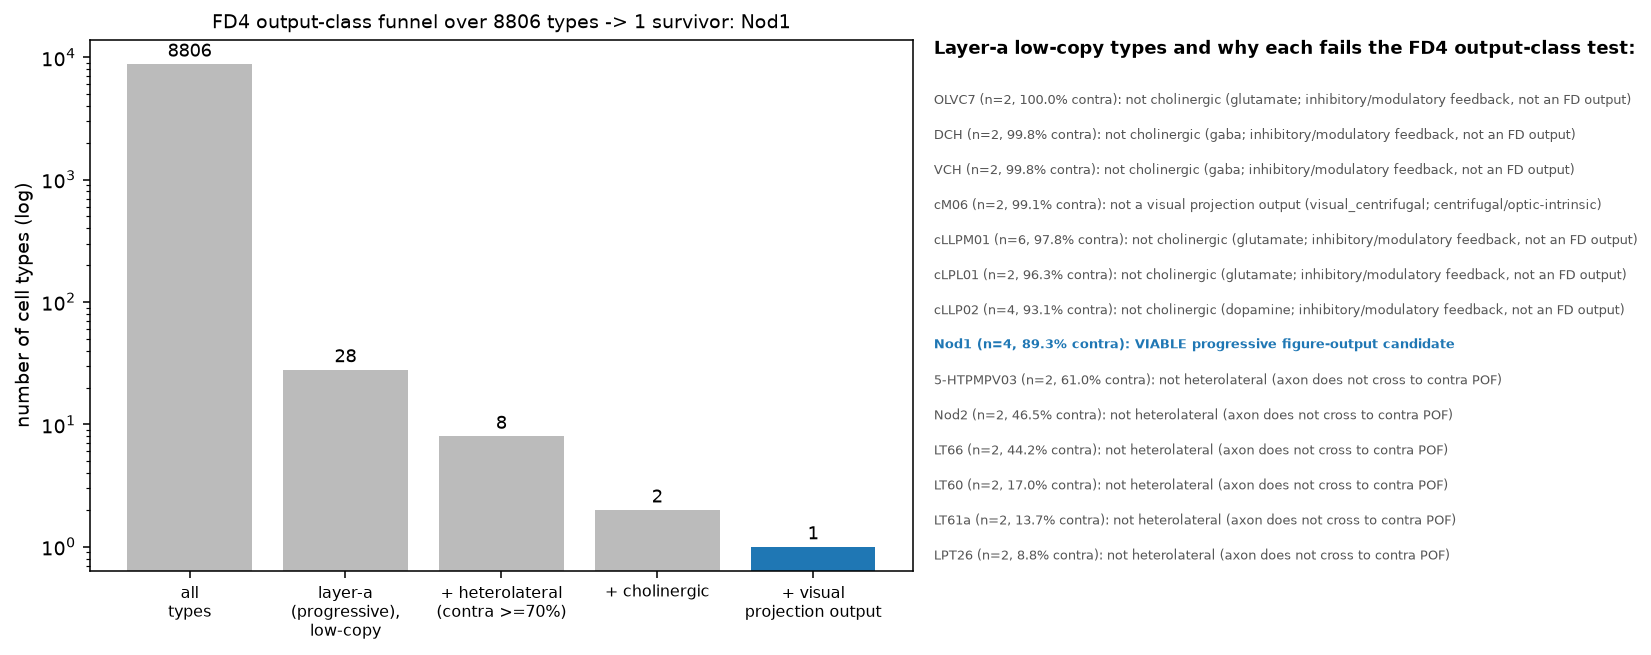
\includegraphics[width=\textwidth]{figures/fd4_candidate_elimination.png}
\caption{\textbf{The candidate elimination.} The FD4 output-class funnel over every FlyWire cell type: progressive (layer-a) and low-copy, then heterolateral, then cholinergic, then a visual projection output. The single survivor is \ttt{Nod1} (= FD1). Each layer-a low-copy type and the reason it fails are listed at right.}\label{fig:elim}
\end{figure}


\paragraph{The \ttt{Nod1} type is one homogeneous population, not FD1 plus FD4.} The FlyWire \ttt{Nod1} type contains four cells, two per hemisphere, where the other FD types contain a single bilateral pair. Egelhaaf described two anatomical FD1 representatives (FD1nod and FD1pof) that were both classed FD1, so a four-cell type is expected to pool two same-side cells. We tested whether those two populations are an FD1 pair and an FD4 pair. They are not. The two same-side cells share a large fraction of their input partners (Jaccard 0.33, against 0.007 across sides), the signature of two copies of one cell type rather than two different cells. Scoring every two-against-two partition of the four cells on the FD4-discriminating features (receptive-field laterality and width, dorso-ventral dendrite extent, and second arbor) isolates no FD4-like pair: the only partition that groups the cells at all is the left-versus-right hemisphere split, a mirror-symmetry effect of the cells' absolute positions rather than a functional FD1 versus FD4 axis, and the more-lateral pair has a larger, not a smaller, dorso-ventral dendrite, the opposite of the FD4 signature. All four cells are frontal, span the full dorso-ventral extent, and have a single arbor. There is no lateral, wide-field, restricted-dendrite FD4 pair inside \ttt{Nod1} (Fig.~\ref{fig:homog}).

\begin{figure}[H]\centering
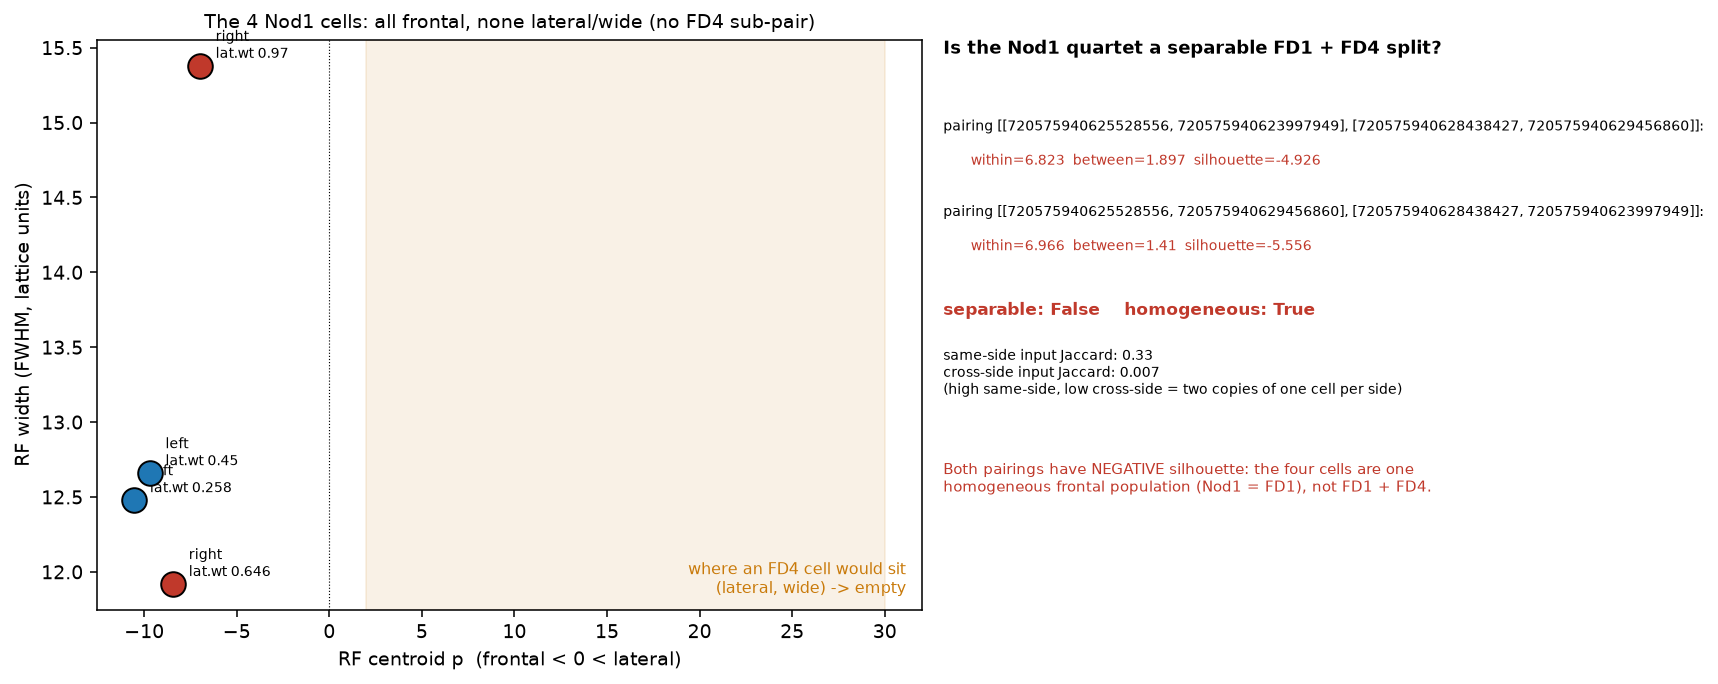
\includegraphics[width=\textwidth]{figures/fd4_nod1_homogeneity.png}
\caption{\textbf{The \ttt{Nod1} quartet is homogeneous.} (left) The four \ttt{Nod1} cells placed by receptive-field centroid (frontal to lateral) and width; all four sit frontally, none in the lateral, wide region an FD4 cell would occupy. (right) The two possible bilateral pairings and their separation scores; both are negative, so the four cells are one population, not a separable FD1 plus FD4 split.}\label{fig:homog}
\end{figure}


\begin{figure}[H]\centering
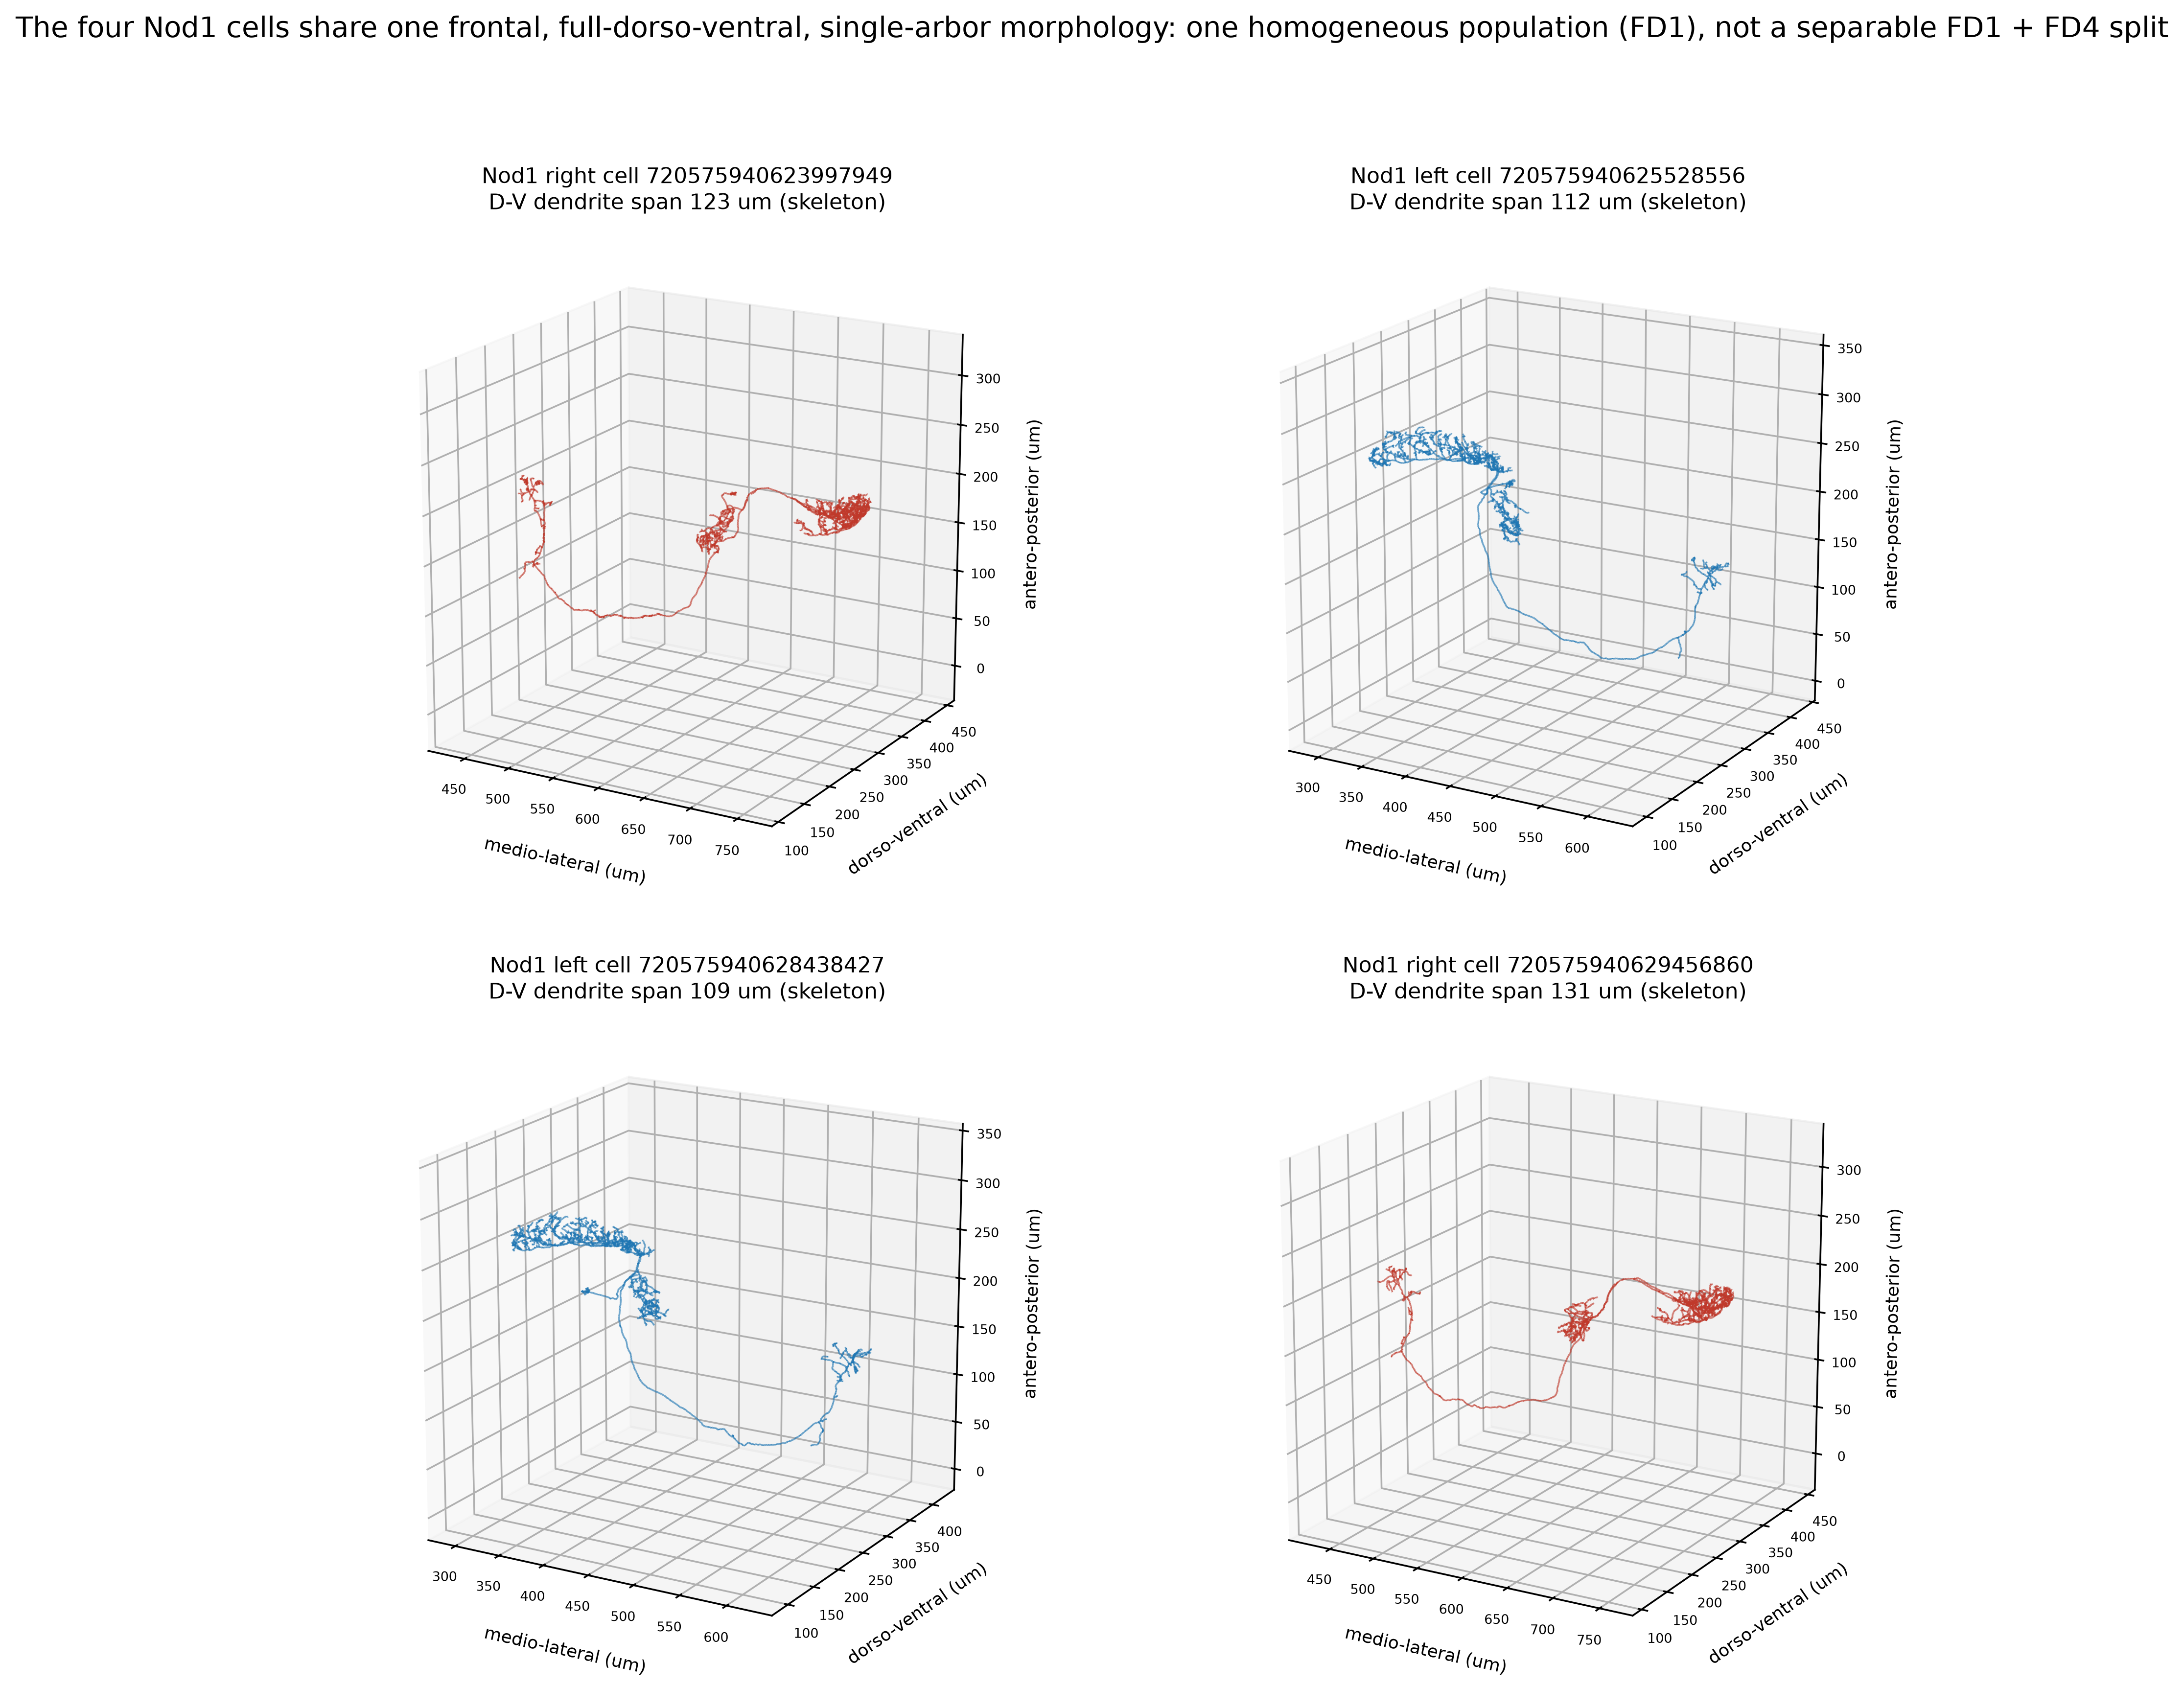
\includegraphics[width=\textwidth]{figures/fd4_nod1_quartet.png}
\caption{\textbf{The four \ttt{Nod1} cells, reconstructed.} Each \ttt{Nod1} cell in anatomical space. All four share one frontal, full-dorso-ventral, single-arbor morphology. An FD1 plus FD4 split would show one pair with a restricted dorso-ventral dendrite; it does not.}\label{fig:quartet}
\end{figure}


\paragraph{What the best candidate does and does not match.} Measuring the FD4-defining properties on the \ttt{Nod1} population (4 of 7 matched) shows the pattern behind the null. The properties it matches are exactly the ones FD4 shares with FD1: progressive direction, heterolateral axon, cholinergic transmitter, and a single arbor. The properties it fails are exactly the ones that would distinguish FD4 from FD1: a whole-eye lateral receptive field, and a restricted dorso-ventral dendrite. In other words, the connectome contains the FD1 half of the FD4 phenotype but not the FD4-specific half (Fig.~\ref{fig:phenotype} and Fig.~\ref{fig:rfcmp}).

\begin{figure}[H]\centering
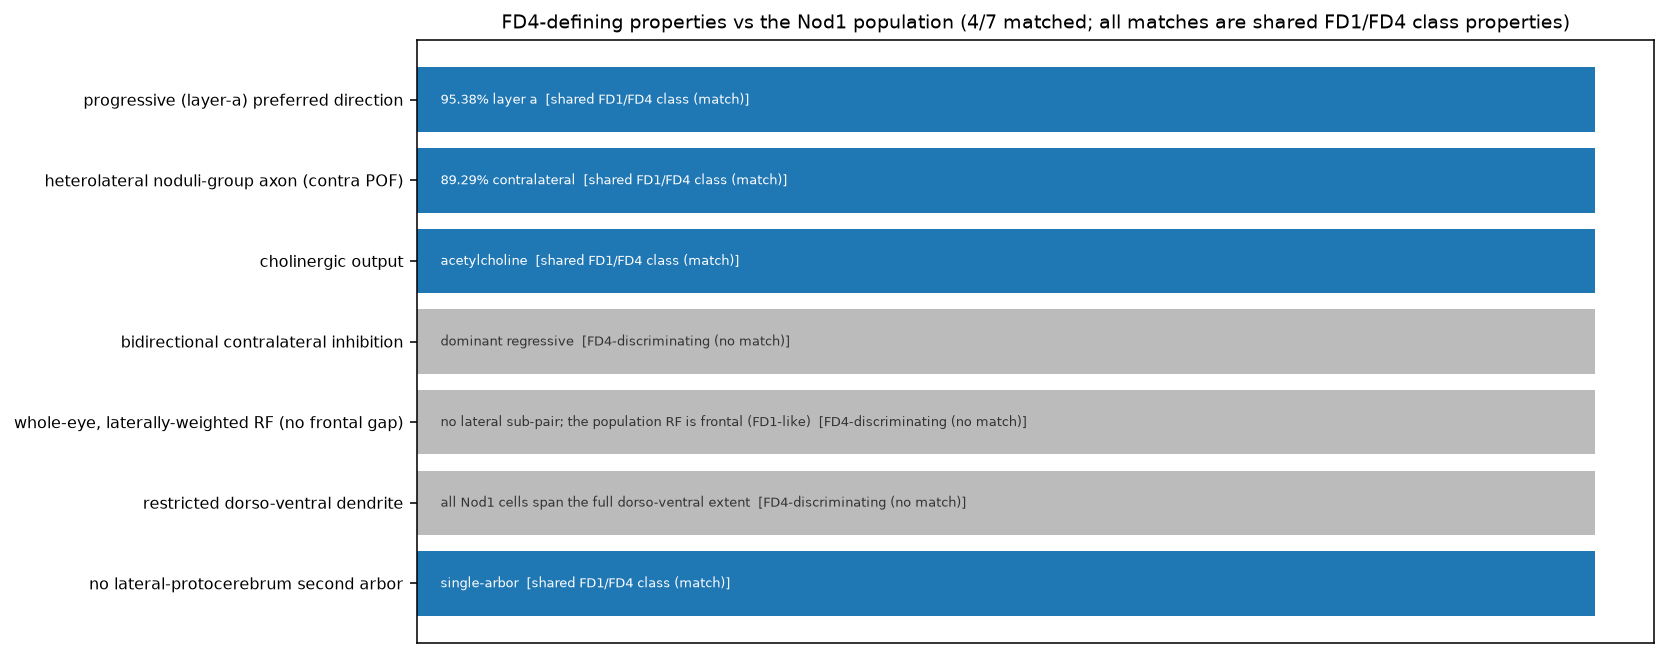
\includegraphics[width=\textwidth]{figures/fd4_phenotype.png}
\caption{\textbf{The FD4 phenotype crosswalk.} Each FD4-defining property and whether the \ttt{Nod1} population matches it. Every match is a property FD4 shares with FD1; every FD4-discriminating property is unmatched.}\label{fig:phenotype}
\end{figure}


\begin{figure}[H]\centering
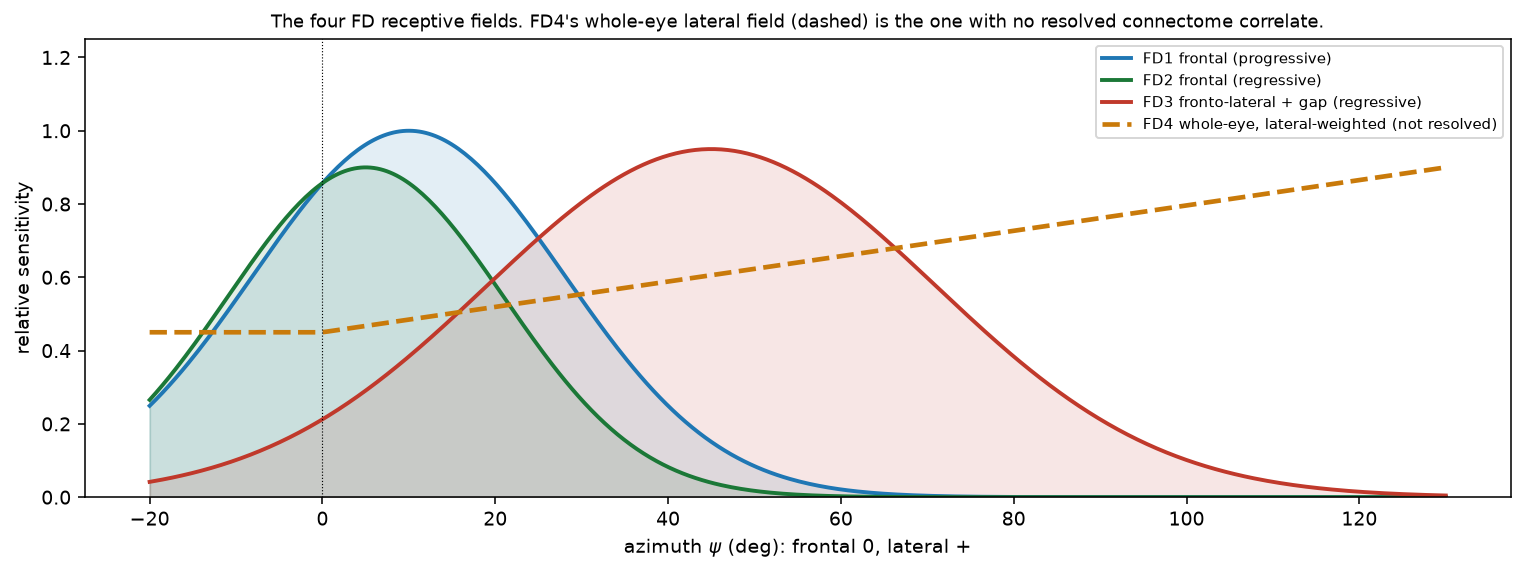
\includegraphics[width=\textwidth]{figures/fd4_rf_comparison.png}
\caption{\textbf{The four FD receptive fields.} FD1 frontal, FD2 frontal, FD3 fronto-lateral with a gap, and FD4 whole-eye and lateral. The measured \ttt{Nod1} field sits frontally with FD1; FD4's whole-eye lateral field (dashed) is the one with no resolved connectome correlate.}\label{fig:rfcmp}
\end{figure}


\begin{figure}[H]\centering
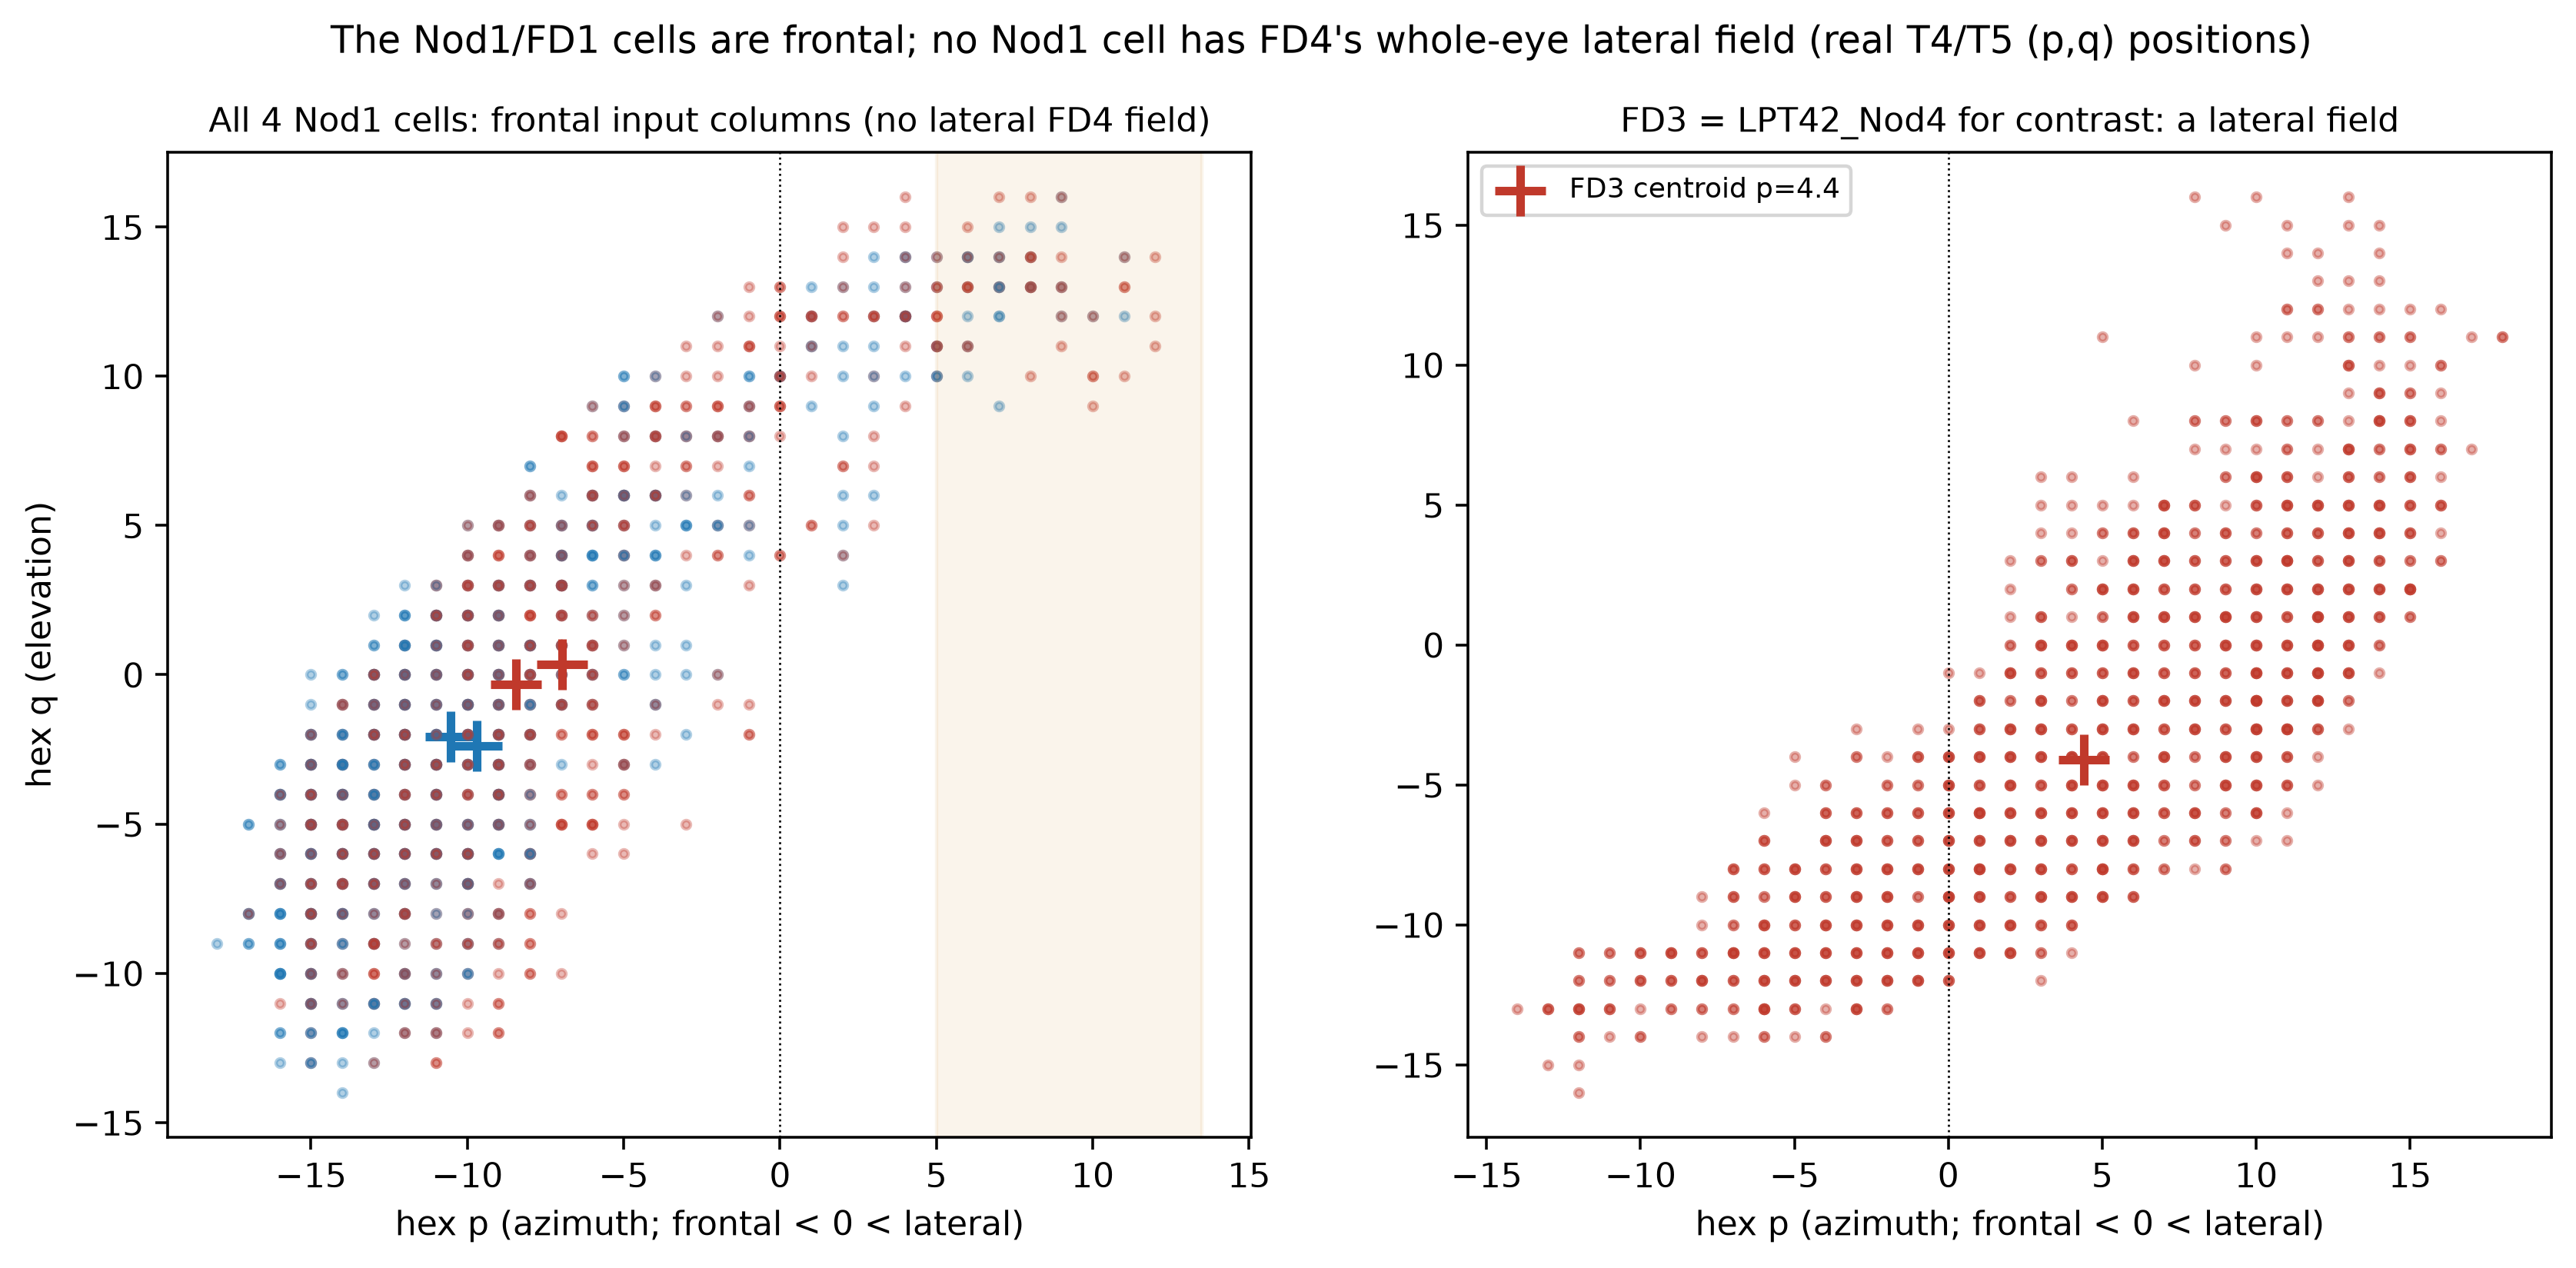
\includegraphics[width=\textwidth]{figures/fd4_input_hexmap.png}
\caption{\textbf{Receptive fields in eye coordinates.} The T4/T5 input columns of each \ttt{Nod1} cell (all frontal) next to \ttt{LPT42\_Nod4} (= FD3, lateral) for contrast. No \ttt{Nod1} cell carries the whole-eye lateral field of FD4.}\label{fig:hexmap}
\end{figure}


\paragraph{The regressive cell that looks FD4-shaped is FD3, not FD4.} The cell \ttt{LPT42\_Nod4}, identified as FD3, has an absolute receptive field that reaches laterally toward the caudal pole and is, on absolute geometry alone, at least as FD4-shaped as FD3-shaped. It is nonetheless FD3, not FD4, because its preferred direction is regressive: 98.58\% of its T4/T5 input is the back-to-front (layer-b) channel, whereas FD4 is progressive (layer-a). Direction is the clean separator. \ttt{LPT42\_Nod4} also has the frontal gap that Egelhaaf certifies as unique to FD3, which FD4 does not have. The FD4-shaped absolute geometry of the FD3 cell is therefore a coincidence of receptive-field position, not an FD4 identity.

\section{Confidence in the result}

The result is expressed as a decomposed, null-aware confidence that FD4 is individually resolved in the connectome, rather than as an assertion either way. It combines the fraction of FD4-\emph{discriminating} properties the best candidate matches (the shared FD1/FD4 class properties carry no power to separate FD4 from FD1 and are excluded from the numerator), a within-\ttt{Nod1} separability factor (zero, because the four cells do not separate into an FD1 and an FD4 population), and explicit discounts. The discounts are larger than for the other FD cells and are stated so a reader can reconstruct the estimate: FD4 shares FD1's entire output class (a collinearity discount of 0.1), FD4 is not an independently annotated FlyWire type (0.07), there is no independent FD4 anchor (0.05), the modern cell-typing authority declined the one-for-one FD1/2/3/4 mapping (0.03), and further FD cells cannot be excluded (0.02). The resulting point estimate is 0.0, with a plausible range of [0.0, 0.27] and a ceiling of 0.85 set by the FD1-collinearity cap (Fig.~\ref{fig:confidence}). The estimate is low and the interval wide by construction: the connectome cannot resolve a cell that shares its entire measurable output class with an already-identified cell and differs only in a receptive field and dendrite extent that are not separately represented in the current annotation.

\begin{figure}[H]\centering
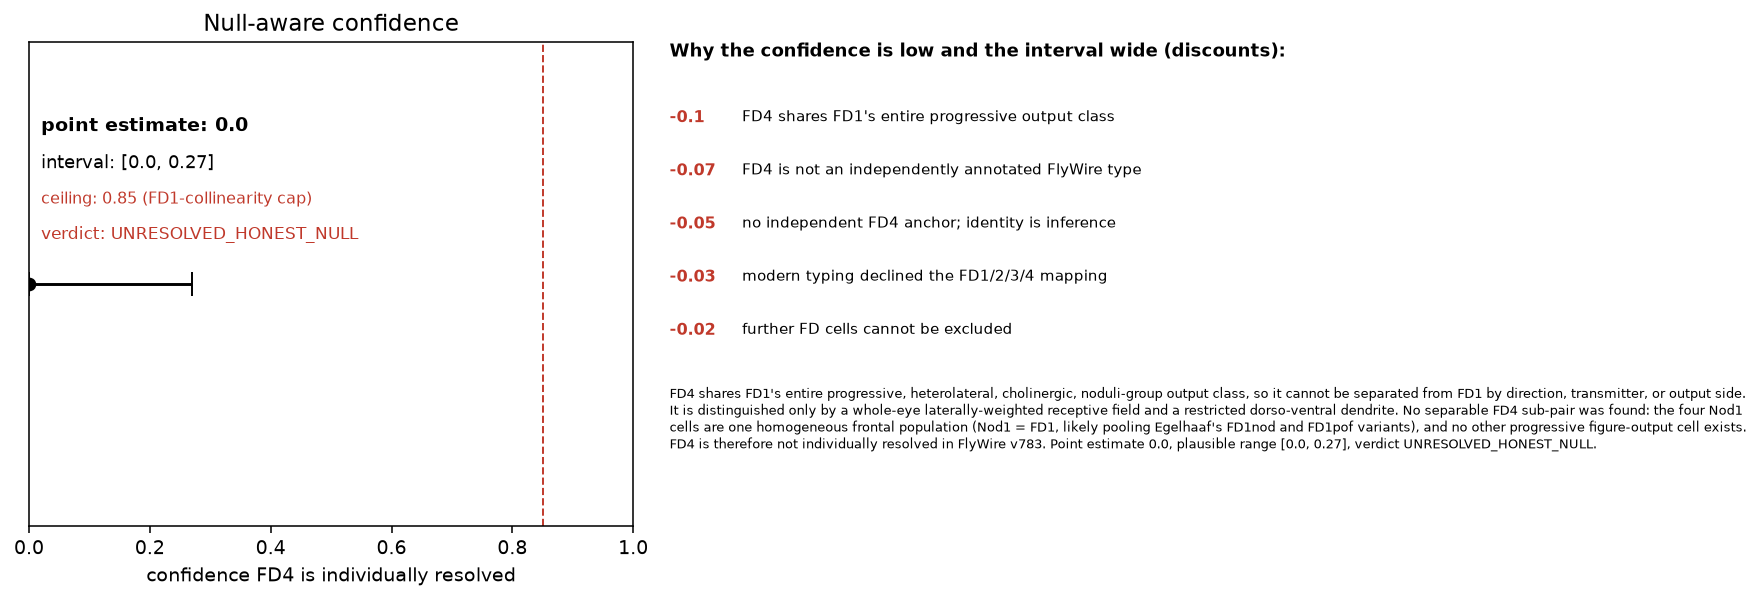
\includegraphics[width=\textwidth]{figures/fd4_confidence.png}
\caption{\textbf{The confidence, decomposed.} (left) The point estimate that FD4 is individually resolved, its wide interval, and the FD1-collinearity ceiling. (right) The discounts that set it, led by the shared-output-class term.}\label{fig:confidence}
\end{figure}


\section{The evidence at a glance}

Table~\ref{tab:evidence} collects the FD4-defining properties and the search tests next to the connectome measurement for each.

\begin{table}[H]\centering\footnotesize\caption{Each defining property of Egelhaaf's FD4 cell and each search test, next to what we find in FlyWire v783.}\label{tab:evidence}

\renewcommand{\arraystretch}{1.25}
\setlength{\tabcolsep}{3pt}
\begin{longtable}{@{}>{\raggedright\arraybackslash}p{0.27\textwidth} >{\raggedright\arraybackslash}p{0.33\textwidth} >{\raggedright\arraybackslash}p{0.34\textwidth}@{}}
\toprule \textbf{FD4 property or test} & \textbf{What Egelhaaf reported} & \textbf{What we find in FlyWire v783} \\\midrule\endhead
Prefers progressive (front-to-back) motion & Egelhaaf: FD4 excited by progressive motion & the progressive figure-output class exists (dominant layer-a), shared with FD1 \\
Whole-eye, laterally-weighted receptive field & Egelhaaf: whole horizontal eye, most sensitive laterally, no gap & not found: all \ttt{Nod1} cells are frontal, none is whole-eye lateral \\
Restricted dorso-ventral dendrite & Egelhaaf: dorso-proximal and ventro-proximal parts devoid of dendrite & not found: all \ttt{Nod1} cells span the full dorso-ventral extent \\
Heterolateral noduli-group axon & Egelhaaf: axon to the contralateral posterior optic foci & present in the \ttt{Nod1} population (shared with FD1 and FD3) \\
Cholinergic output & FD cells are excitatory output neurons & acetylcholine (shared with FD1) \\
Bidirectional contralateral inhibition & Egelhaaf: FD4 inhibited by contra motion in either direction (FD1 unidirectional) & the one FD1-versus-FD4 discriminator not exhausted within \ttt{Nod1} (see caveats) \\
A separate progressive figure-output cell & the identification requires a distinct cell & none: \ttt{Nod1} is the sole survivor of the output-class funnel \\
A separable FD4 sub-pair of \ttt{Nod1} & a four-cell type could pool FD1 and FD4 & none: the four cells are homogeneous (no partition isolates an FD4-like pair; separable = False) \\
The FD4-shaped regressive cell is not FD4 & FD4 is progressive; the frontal gap is FD3-unique & \ttt{LPT42\_Nod4} is 98.58\% layer-b (regressive) = FD3, not FD4 \\
Confidence FD4 is individually resolved & quantify the result honestly & point 0.0, range [0.0, 0.27], verdict UNRESOLVED\_HONEST\_NULL \\
\bottomrule\end{longtable}
\renewcommand{\arraystretch}{1.0}
\setlength{\tabcolsep}{6pt}

\end{table}

\section{What the data can and cannot settle}

\textbf{The result is a negative one, stated as such.} No cell in FlyWire v783 carries the FD4-specific receptive field and dendrite together with the progressive noduli-group output class. This is reported as a null result rather than forced into an identification. \textbf{FD4 shares FD1's entire measurable output class.} Preferred direction, output side, and transmitter, the three connectome signatures that identify an FD output cell, are identical for FD1 and FD4. The connectome can therefore locate the progressive figure-output class but cannot, from these signatures alone, split it into FD1 and FD4. \textbf{The distinguishing features are not separately represented.} FD4 differs from FD1 in receptive-field width and laterality and in dorso-ventral dendrite extent; measured on the \ttt{Nod1} cells, these do not separate the population, so either the FD4 cell is not reconstructed as distinct in this annotation, or it is pooled within \ttt{Nod1} below the resolution of these measurements. \textbf{The receptive-field axis is relative.} The frontal reading of the \ttt{Nod1} cells is made relative to the FD3 cell in the same coordinate frame and gives the correct FD1-frontal, FD3-lateral ordering, so it does not depend on an absolute azimuth calibration. \textbf{The modern typing declined the FD mapping.} The cell-typing authority that named these cells stated that the FD cells are almost certainly homologous to noduli-group cells but did not establish one-for-one FD1/2/3/4 matches; every FD assignment in this program, including the FD1 anchor this search rests on, is a derived correlate, not a literature-endorsed identity. \textbf{One FD1-versus-FD4 discriminator was not exhausted.} Beyond receptive field and dendrite, Egelhaaf gives one further property that separates FD4 from FD1 and is in principle connectome-measurable: FD4 is inhibited by contralateral motion in either direction (bidirectional), whereas FD1 is reduced only by contralateral regressive motion (unidirectional). This is an inhibitory-input property, not one of the shared output-class signatures, and a targeted search for a bidirectionally contra-inhibited subset within \ttt{Nod1} was not carried out here. It is the one avenue by which a distinct FD4 could yet be resolved, and it is left open rather than claimed either way. \textbf{Every load-bearing claim was tested adversarially.} The candidate elimination, the \ttt{Nod1} homogeneity, the FD1-collinearity, the receptive-field axis, the exclusion of the FD4-shaped FD3 cell, the Nod-family siblings, and the confidence interval were each subjected to an independent attempt at refutation with fresh connectome queries; all seven survived, and the residual caveats surfaced there, including the bidirectional-inhibition avenue above, are the ones stated in this report.

\clearpage

\part{Inputs: the progressive figure arm}

\textbf{Summary.}\quad Although FD4 is not individually resolved, the progressive figure arm that any FD4 correlate would use is fully present in the connectome and is traced here on the \ttt{Nod1} (= FD1) population. It reads front-to-back (layer-a) motion from the T4a and T5a detectors (95.38\% of its T4/T5 drive is layer-a), relays it through a columnar projection sheet, and is gated by wide-field inhibitory cells. This is the progressive mirror of the regressive FD2 and FD3 arms.

\section{The motion detectors that drive the progressive arm}

The progressive figure arm reads the front-to-back (layer-a) motion channel: 95.38\% of its T4/T5 input is layer-a, carried by both the ON detector \ttt{T4a} and the OFF detector \ttt{T5a} (ON/OFF split \{'T4a\_ON': 955, 'T5a\_OFF': 1109, 't4\_frac': 46.3\}). This is the opposite motion channel from FD2 and FD3, which read the regressive (layer-b) detectors, and it matches the progressive direction Egelhaaf reported for FD1 and FD4 (Fig.~\ref{fig:census}).

\begin{figure}[H]\centering
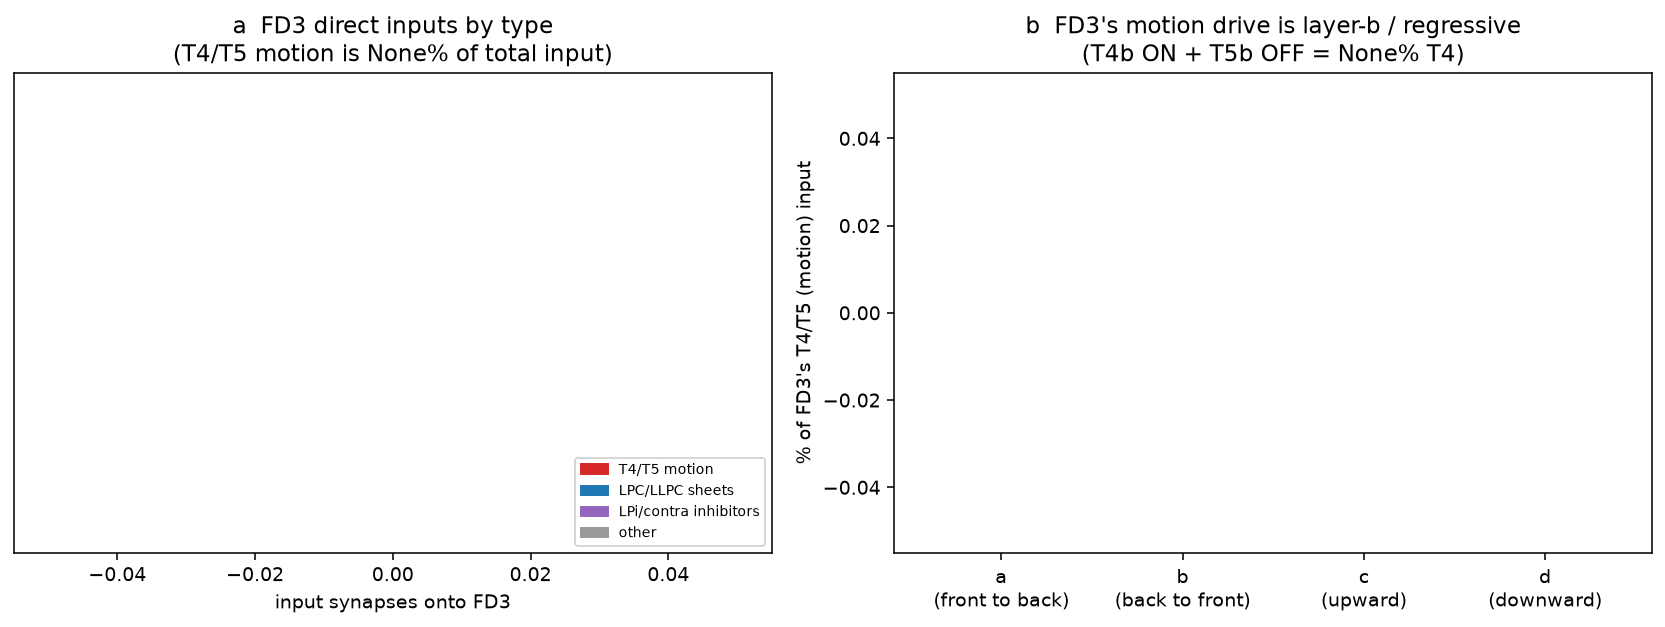
\includegraphics[width=\textwidth]{figures/fd4_input_census.png}
\caption{\textbf{What feeds the progressive figure cell.} The direct inputs of \ttt{Nod1}, coloured by class, with the front-to-back (layer-a) T4a/T5a motion detectors marked. This is the arm any FD4 correlate would read.}\label{fig:census}
\end{figure}


\section{From the eye to the detectors}

The T4a and T5a cells that drive the progressive arm are fed by the canonical ON and OFF medulla cells, which are fed by the lamina and, before it, the photoreceptors. The whole cascade from the eye to the detectors is present in the connectome and matches published optic-lobe wiring (lamina present: ['L1', 'L2', 'L3', 'L4', 'L5']; photoreceptors: ['R1-6', 'R7', 'R8']). This cascade is the general column-to-column wiring of the optic lobe, the pathway that culminates in the progressive detectors, not a per-object trace.

\section{Where the input lands, and the sheet and gate}

Each motion detector looks at one point in the eye, so the detectors feeding the progressive cell draw out its receptive field on the eye's lattice; for the \ttt{Nod1} population this field is frontal (Fig.~\ref{fig:hexmap2}). The motion detectors also reach the cell through a columnar projection sheet, the layer-a sheet \ttt{LLPC1}, and the cell is gated by wide-field inhibitory cells led by \ttt{LPi15}. This is the same sheet-and-gate architecture as the FD1 arm, as expected for a progressive figure cell (Fig.~\ref{fig:arbor}).

\begin{figure}[H]\centering
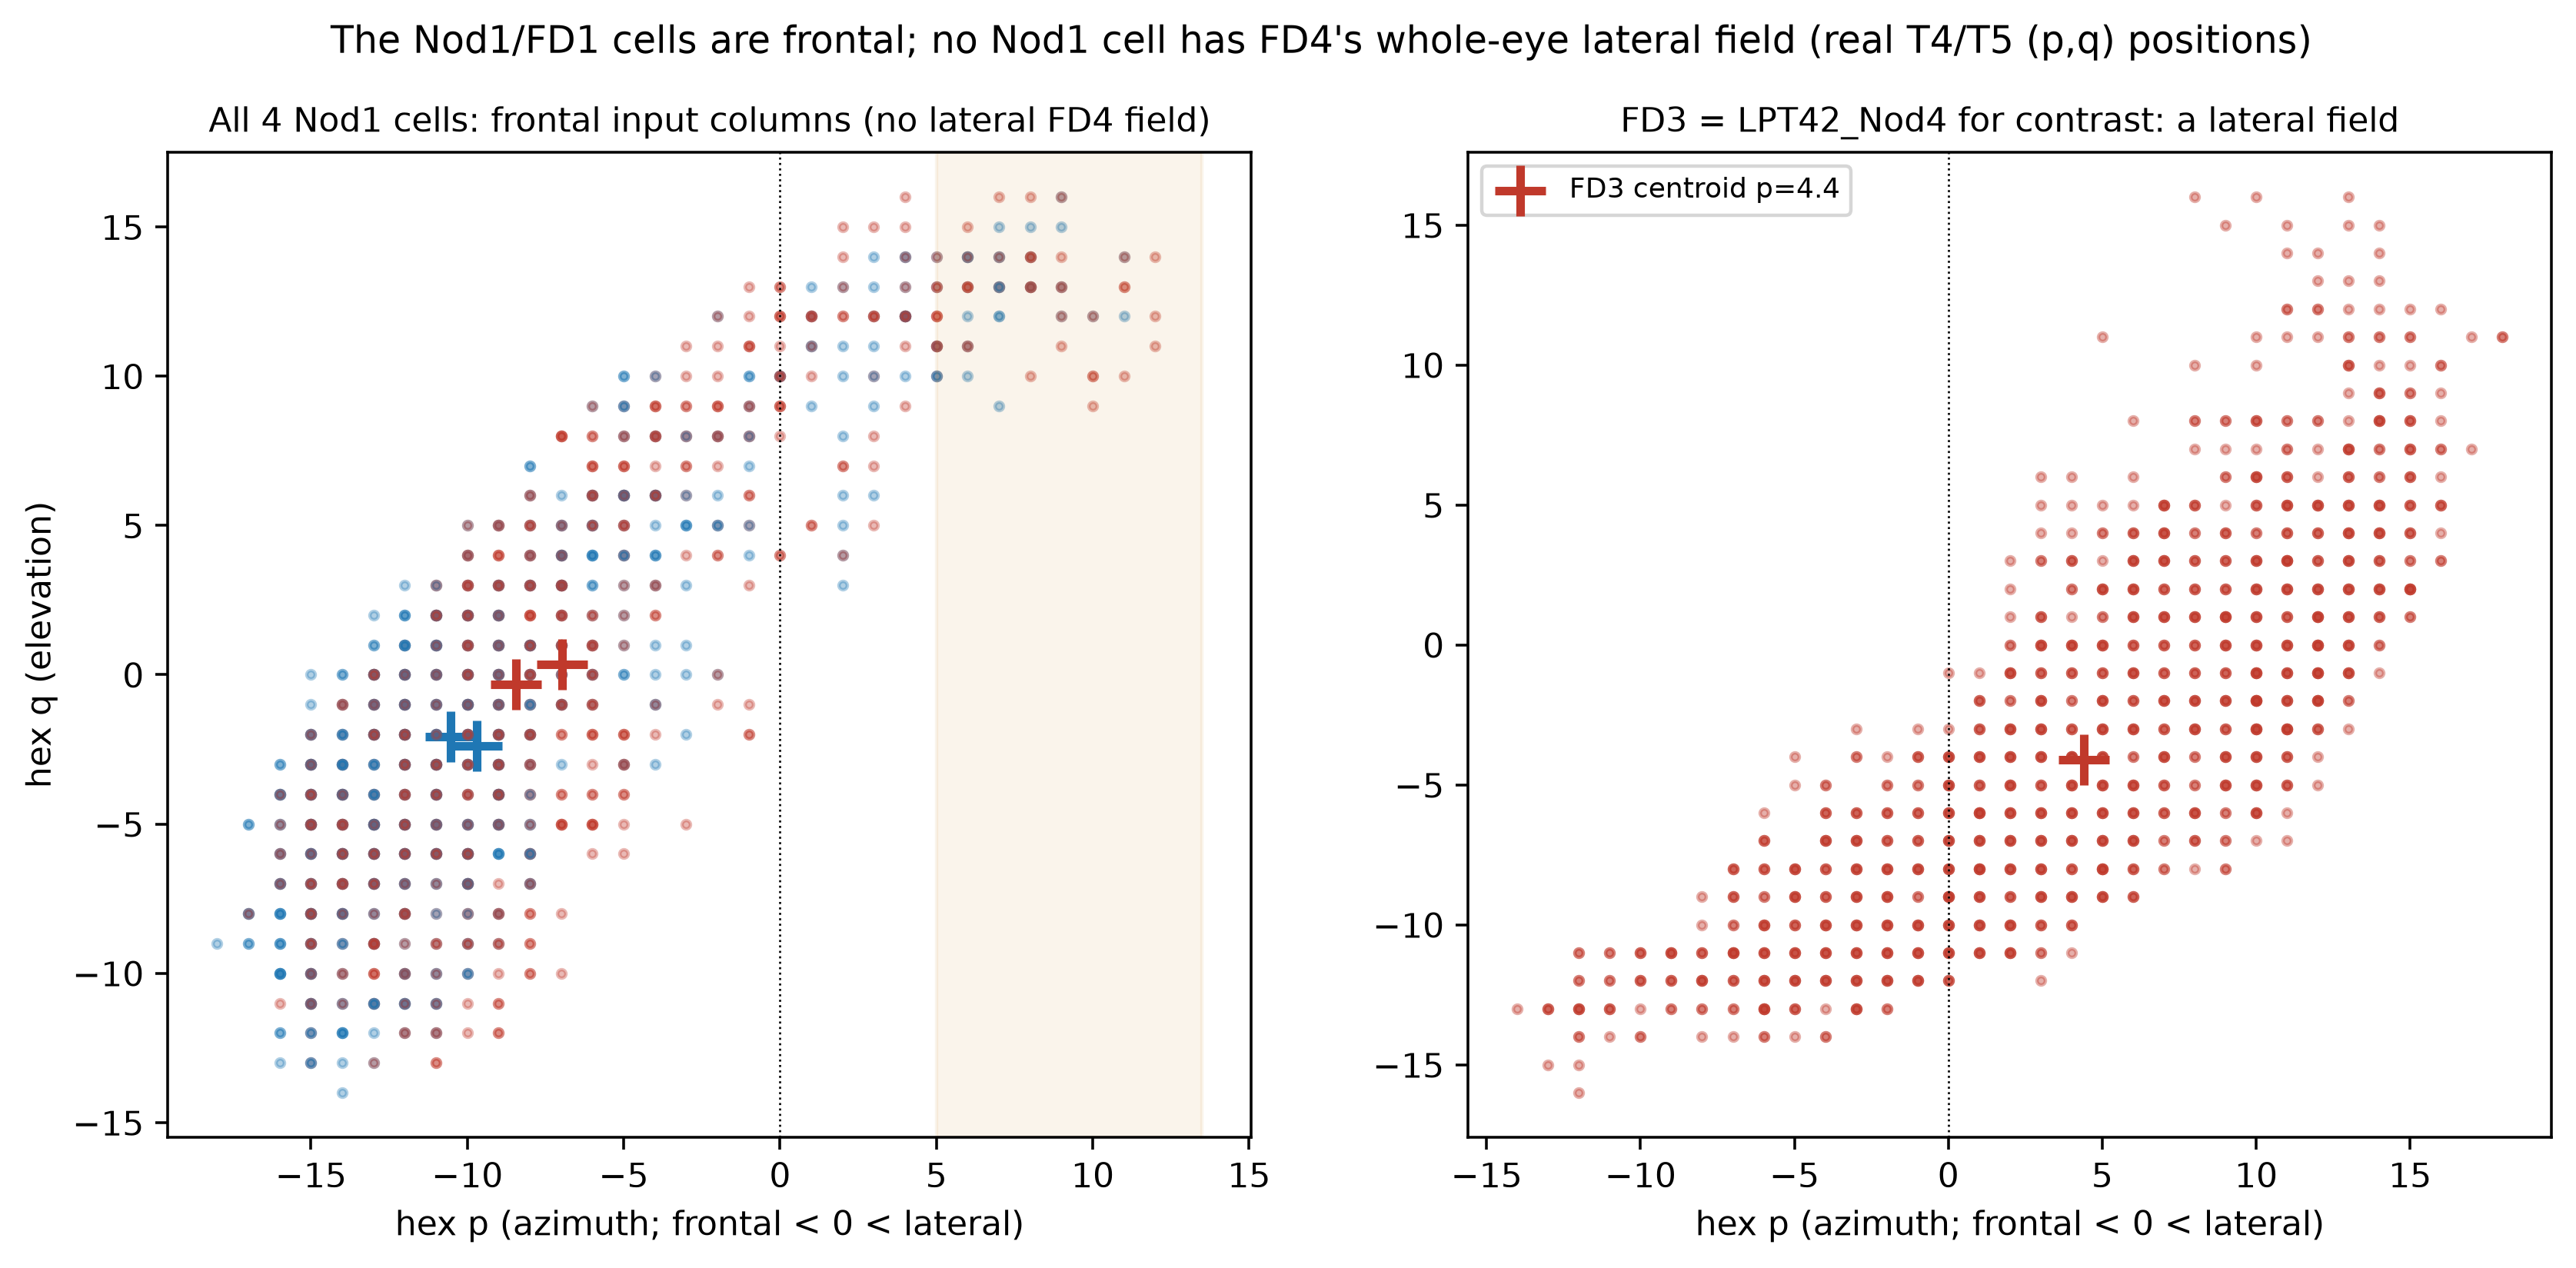
\includegraphics[width=\textwidth]{figures/fd4_input_hexmap.png}
\caption{\textbf{The progressive arm's input in eye coordinates.} The T4/T5 input columns of the \ttt{Nod1} cells (frontal) and \ttt{LPT42\_Nod4} (= FD3, lateral) for contrast.}\label{fig:hexmap2}
\end{figure}


\begin{figure}[H]\centering
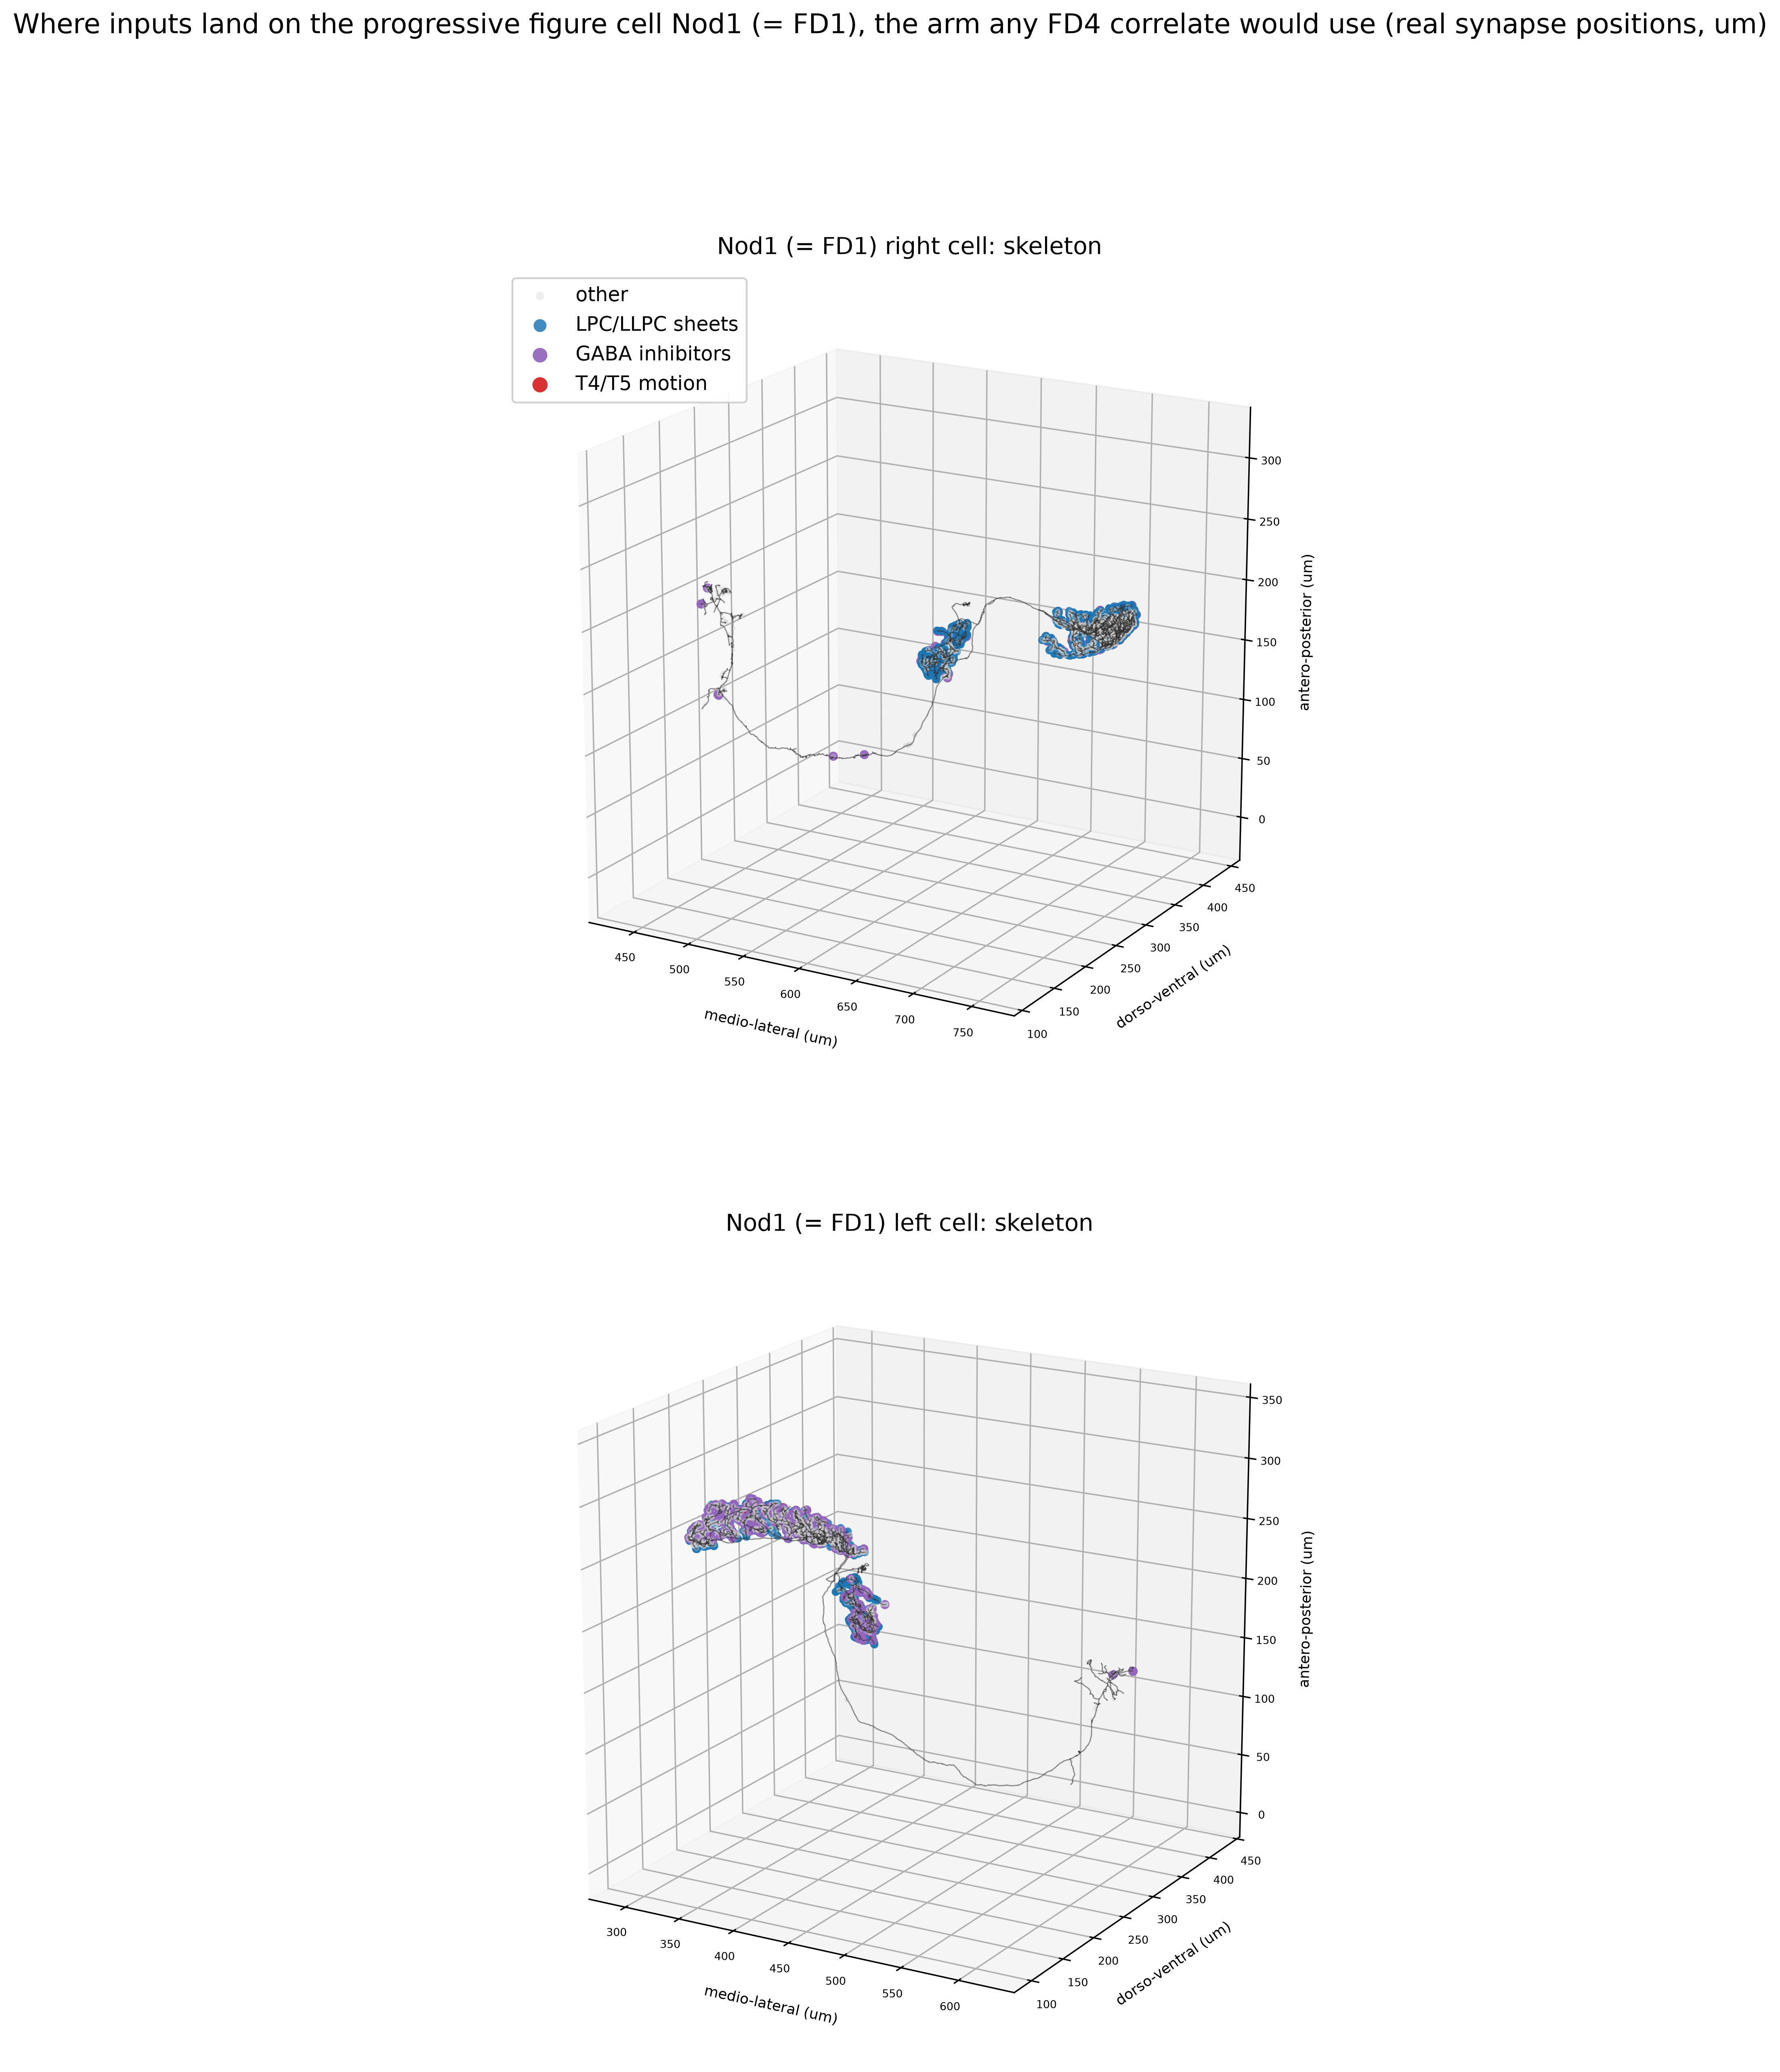
\includegraphics[width=\textwidth]{figures/fd4_arbor_inputs.png}
\caption{\textbf{Inputs on the progressive cell's arbor.} Each \ttt{Nod1} cell's reconstructed shape with its input synapses drawn at their real positions and coloured by the class of partner: front-to-back motion detectors, columnar sheets, and inhibitory cells.}\label{fig:arbor}
\end{figure}


\section{What the data can and cannot settle}

\textbf{The arm is traced on FD1, not on a resolved FD4.} Because FD4 is not individually resolved, the afferent trace is measured on the \ttt{Nod1} (= FD1) population, which uses the same progressive channel, sheet, and gate any FD4 correlate would. It is shown as the realized progressive figure arm, not as an FD4-specific trace. \textbf{The upstream cascade is general wiring.} The photoreceptor-to-detector cascade is measured cell-type by cell-type across the optic lobe and matches the known column wiring.

\clearpage

\part{Outputs: descending and motor-system partners}

\textbf{Summary.}\quad The progressive figure arm reaches descending neurons that project into the ventral nerve cord and contact motor-control networks. Traced on the \ttt{Nod1} population, its leading direct descending target is \ttt{DNp26}, the same wing-steering command neuron that the FD2 and FD3 arms reach, so the figure cells converge on a shared descending target. Any FD4 correlate, sharing this arm, would reach the same steering pathway.

\section{The descending neurons the progressive arm contacts}

\ttt{Nod1} makes 453 output synapses onto 8 descending-neuron types, led by \ttt{DNp26} (Fig.~\ref{fig:dnrank}). \ttt{DNp26} is the convergent wing-steering command neuron shared with the FD2 and FD3 arms. Egelhaaf could name only ``descending neurones'' generically; the connectome names them.

\begin{figure}[H]\centering
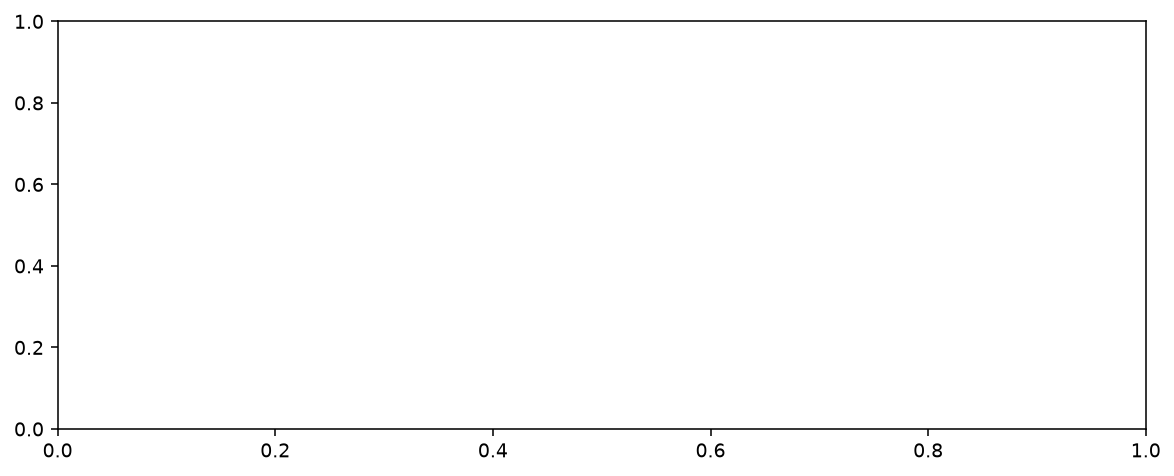
\includegraphics[width=\textwidth]{figures/fd4_dn_ranking.png}
\caption{\textbf{The descending neurons the progressive arm contacts.} Each bar is one descending-neuron type, ranked by synapses received from \ttt{Nod1}. Red marks neurons known to drive wing-steering muscles.}\label{fig:dnrank}
\end{figure}


\section{Motor systems contacted by those neurons}

Following each descending neuron into the male nerve-cord connectome and weighting by how strongly the progressive cell drives it, the descending output is biased toward the wing-steering motor system (dominant system: \ttt{wing\_steering}; Fig.~\ref{fig:motorsys}). As in the FD2 and FD3 reports, the label is by descending-neuron identity; weighting by actual muscle targets softens the picture toward a mixed steering and neck-gaze bias, and the contact is sparse. The pathway supports a steering role, consistent with Egelhaaf's proposal that the FD cells contribute to yaw-torque control, but does not by itself prove a behaviour.

\begin{figure}[H]\centering
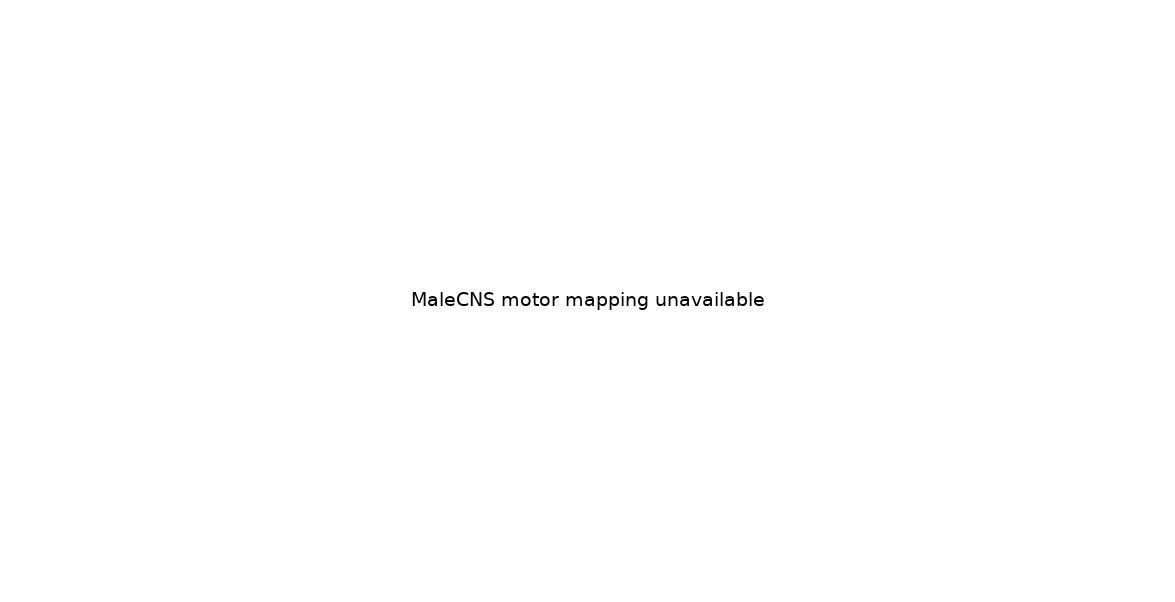
\includegraphics[width=\textwidth]{figures/fd4_motor_systems.png}
\caption{\textbf{Motor-system proxy.} The motor systems reached by the progressive arm's descending output, weighted by how strongly the cell drives each descending neuron. Wing-steering has the largest share.}\label{fig:motorsys}
\end{figure}


\section{The circuit in the brain}

Seen alongside the cells it connects, the progressive figure cell sits anatomically between the lobula-plate motion detectors and the descending neurons that contact wing-steering motor systems (Fig.~\ref{fig:circuit3d}).

\begin{figure}[H]\centering
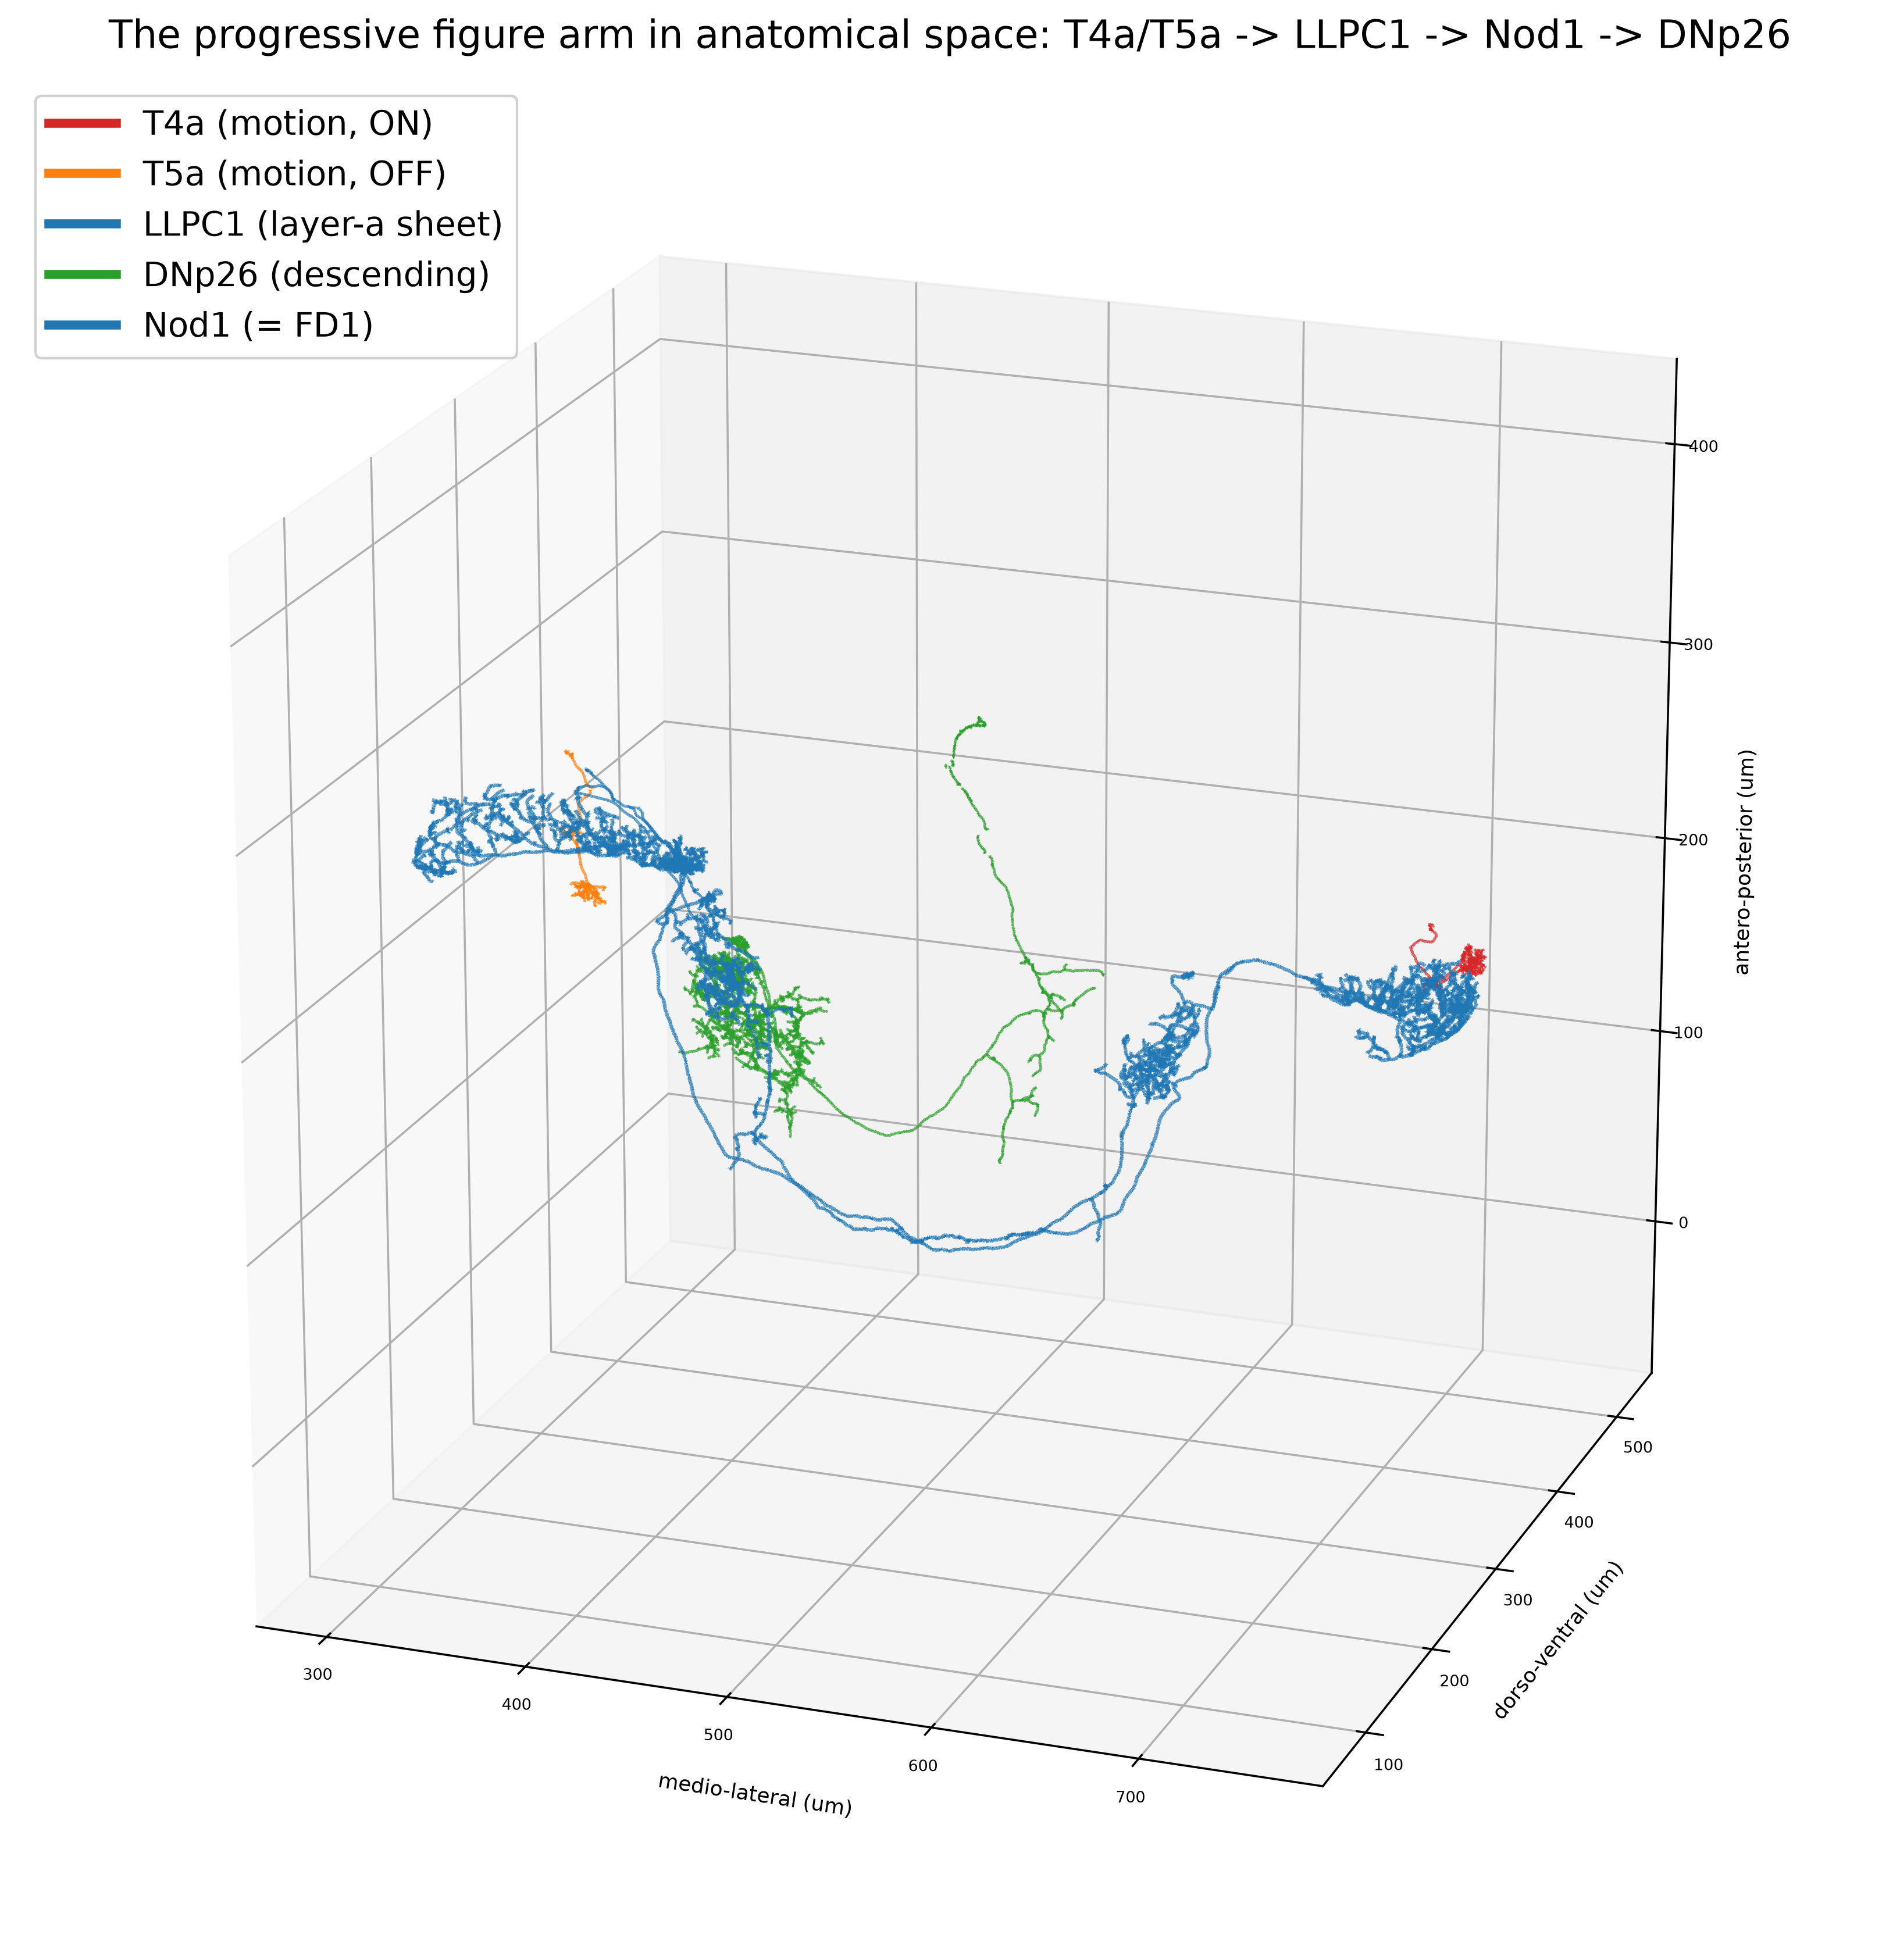
\includegraphics[width=\textwidth]{figures/fd4_circuit_3d.png}
\caption{\textbf{The progressive arm in the brain.} Reconstructed neurons of the progressive figure arm in their true anatomical positions: the \ttt{T4a}/\ttt{T5a} motion detectors, the layer-a sheet, the \ttt{Nod1} cells, and the descending neuron they lead to.}\label{fig:circuit3d}
\end{figure}


\section{What the data can and cannot settle}

\textbf{The output is traced on FD1.} As on the input side, the efferent trace is measured on the \ttt{Nod1} population because FD4 is not individually resolved; it is the realized progressive-arm output, which any FD4 correlate would share. \textbf{The steering label is by neuron identity, not muscle count}, and \textbf{the muscle map crosses two connectomes} by shared descending-neuron name, as in the FD2 and FD3 reports.

\clearpage

\part{The functional figure-ground circuit of the progressive arm}

\textbf{Summary.}\quad This part names the working progressive figure-ground circuit, in the same terms as the FD1, FD2, and FD3 arms: front-to-back motion detectors to the layer-a sheet \ttt{LLPC1} to the progressive figure cell to the steering neuron \ttt{DNp26}, gated by the wide-field inhibitor \ttt{LPi15}. This is the circuit an FD4 correlate would occupy.

\section{The progressive cell's connectivity, comprehensively}

The \ttt{Nod1} population receives about 14314 input synapses from roughly 2750 partner cells, and makes about 24308 output synapses onto roughly 13028 partners. The inputs are dominated by the motion detectors, the columnar sheets, and inhibitory cells; the outputs reach central brain cells and, through the descending neurons, the steering muscles (Fig.~\ref{fig:wheel}).

\begin{figure}[H]\centering
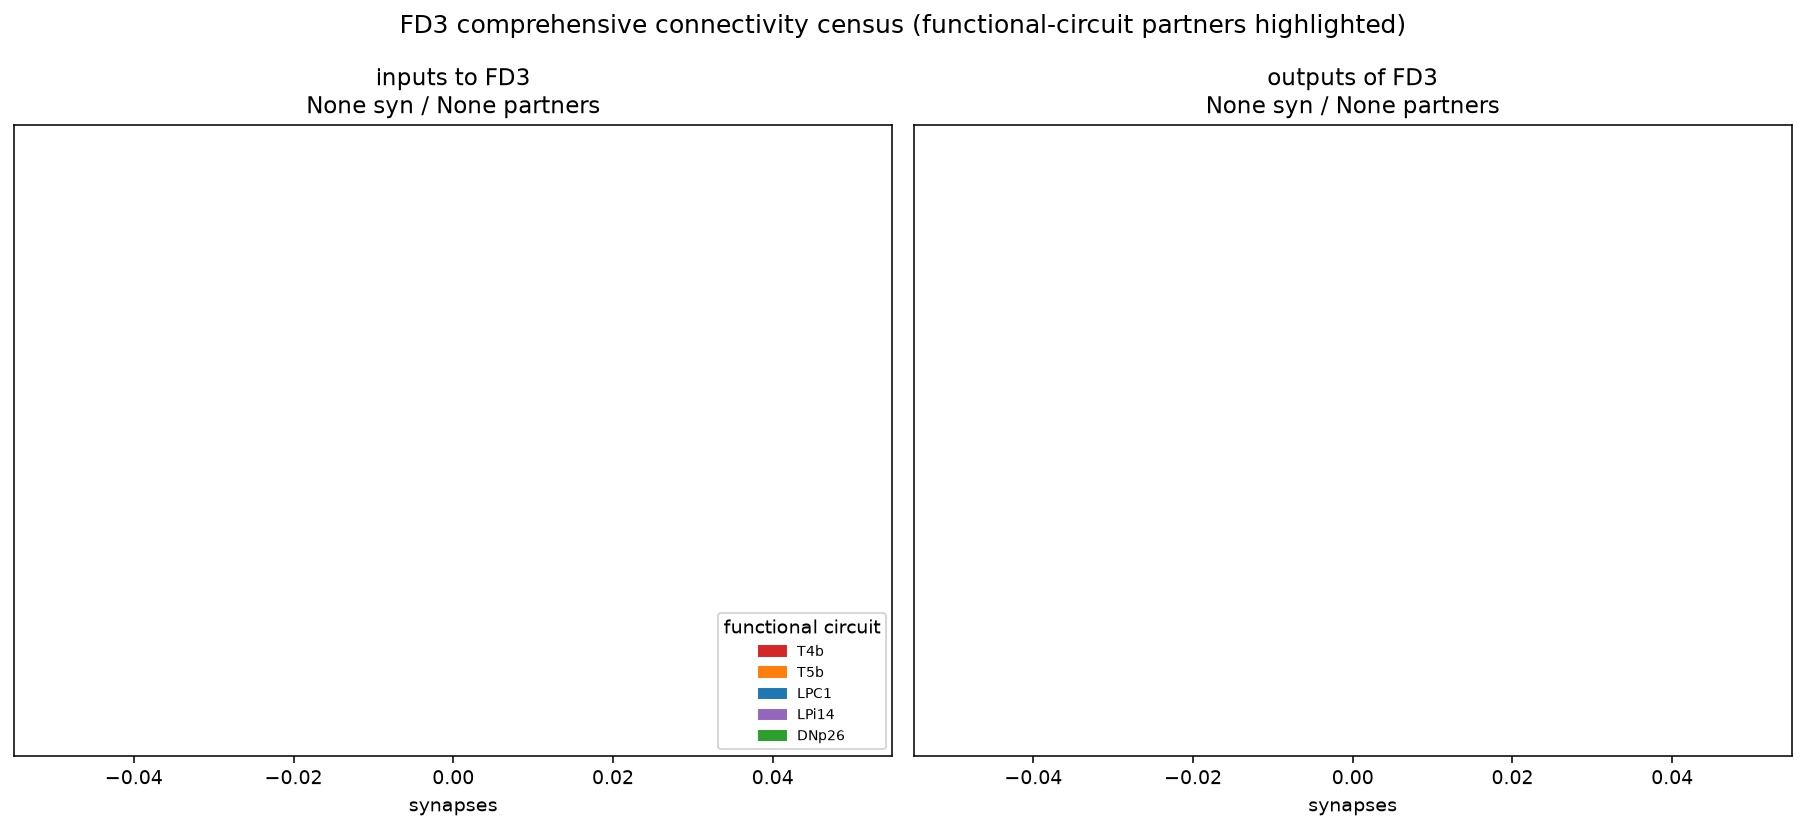
\includegraphics[width=\textwidth]{figures/fd4_connectivity_wheel.png}
\caption{\textbf{The progressive cell's comprehensive connectivity.} Every major input (left) and output (right) partner type of \ttt{Nod1}.}\label{fig:wheel}
\end{figure}


\section{The circuit, named end to end}

Putting the pieces together, the progressive figure-ground circuit reads: the \ttt{T4a}/\ttt{T5a} front-to-back motion detectors drive the layer-a sheet \ttt{LLPC1}, which relays to the progressive figure cell; the cell drives the steering command neuron \ttt{DNp26} and thence the wing; and the wide-field cell \ttt{LPi15} gates the circuit. This is the same architecture as the FD1, FD2, and FD3 arms, built from the progressive channel. FD4, if it were individually resolved, would be a second progressive figure cell reading this same arm with a wider, more lateral receptive field. The connectome contains the arm but not a second cell reading it (Fig.~\ref{fig:funcircuit}).

\begin{figure}[H]\centering
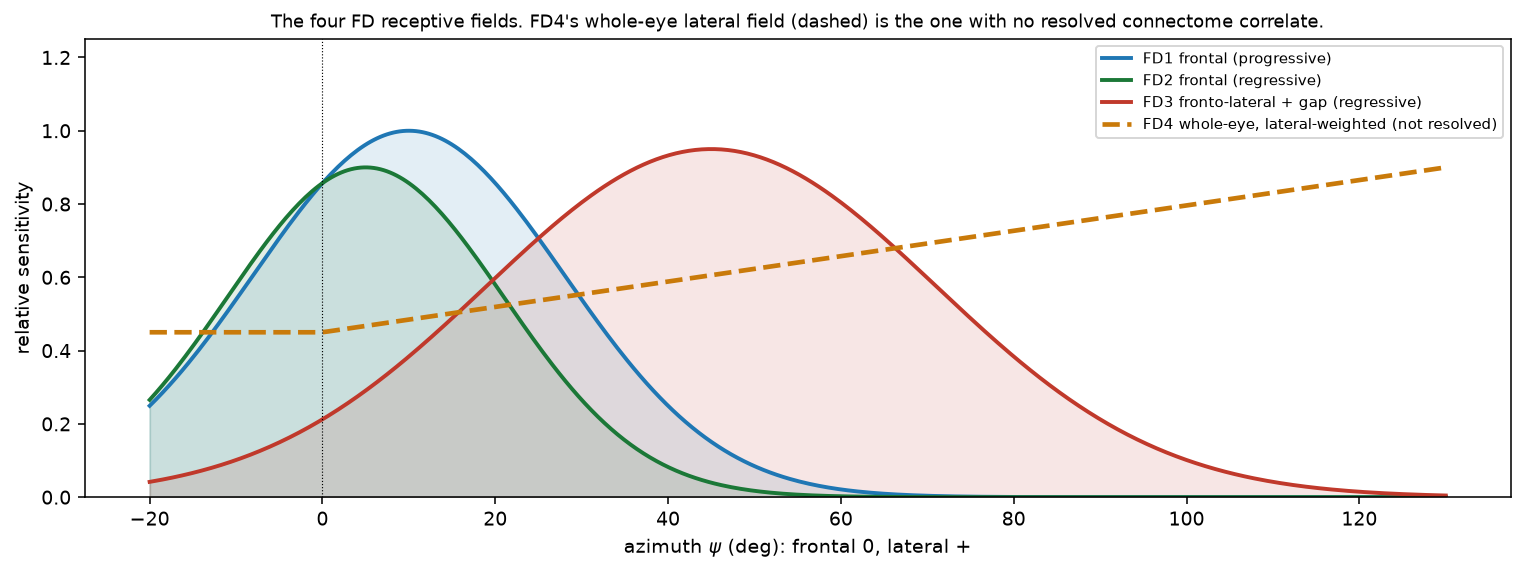
\includegraphics[width=\textwidth]{figures/fd4_rf_comparison.png}
\caption{\textbf{Where FD4 would sit.} The four FD receptive fields on one eye's azimuth axis. FD4's whole-eye lateral field (dashed) is the position a second progressive figure cell would occupy; it has no resolved connectome correlate.}\label{fig:funcircuit}
\end{figure}


\section{What the data can and cannot settle}

\textbf{Sign is not read from wiring.} That a GABAergic contact is inhibitory, and that the gate shapes the figure response, are expectations from physiology; the connectome supplies the connections, not the sign. \textbf{The circuit is the FD1 arm.} It is named as the progressive figure arm any FD4 correlate would use, not as an FD4-specific circuit, because no distinct FD4 cell is resolved.

\section{Methods and provenance}

\textbf{Connectome.} FlyWire FAFB materialization v783 (\ttt{synapses\_nt\_v1}, no cleft threshold), track \ttt{offline}. The \ttt{Nod1} homogeneity finding, the load-bearing negative result, was checked across the offline, live, and v630 tracks (tracks: ['offline', 'live', 'v630']). Neuron annotations are the Schlegel/Codex tables. \textbf{Candidate elimination} funnels every cell type by dominant lobula-plate layer, output laterality, transmitter, and copy number, using the per-type scan of all FlyWire types. \textbf{Preferred direction} is the synapse-weighted T4/T5 lobula-plate layer composition~\cite{fd1989,maisak2013}. \textbf{Receptive field}: T4/T5 inputs carry hex-lattice coordinates; each \ttt{Nod1} cell's field is measured per cell and compared in the shared frame. \textbf{The \ttt{Nod1} split} enumerates the two bilateral pairings of the four cells and scores each on receptive-field laterality and width, dorso-ventral dendrite extent, and second-arbor bimodality; a positive split requires a positive separation score and an FD4-featured pair. \textbf{Confidence} combines the discriminating-property match fraction, the within-\ttt{Nod1} separability, and explicit discounts led by the FD1-collinearity term. \textbf{Afferent, sheet, gate, efferent} reuse the FD-circuit machinery parameterised on the progressive (layer-a) arm and the \ttt{Nod1} population; the motor read-out crosses into the male CNS by shared descending-neuron name. \textbf{Reproducibility}: built from the FD4 verification JSON.

\clearpage

\begin{thebibliography}{11}
\bibitem{egelhaaf1985a} Egelhaaf M. (1985) On the neuronal basis of figure-ground discrimination by relative motion in the visual system of the fly. I. \textit{Biol. Cybern.} 52:123--140.
\bibitem{egelhaaf1985b} Egelhaaf M. (1985) \ldots II. Figure-detection cells, a new class of visual interneurones. \textit{Biol. Cybern.} 52:195--209. (FD4 at pp.~204--206.)
\bibitem{egelhaaf1985c} Egelhaaf M. (1985) \ldots III. Possible input circuitries and behavioural significance of the FD-cells. \textit{Biol. Cybern.} 52:267--280.
\bibitem{rp1979} Reichardt W., Poggio T. (1979) Figure-ground discrimination by relative movement in the visual system of the fly. I. \textit{Biol. Cybern.} 35:81--100.
\bibitem{fd1989} Fischbach K.-F., Dittrich A.P.M. (1989) The optic lobe of \textit{Drosophila melanogaster}. I. A Golgi analysis of wild-type structure. \textit{Cell Tissue Res.} 258:441--475.
\bibitem{maisak2013} Maisak M.S. et al. (2013) A directional tuning map of \textit{Drosophila} elementary motion detectors. \textit{Nature} 500:212--216.
\bibitem{namiki2018} Namiki S. et al. (2018) The functional organization of descending sensory-motor pathways in \textit{Drosophila}. \textit{eLife} 7:e34272.
\bibitem{dorkenwald2024} Dorkenwald S. et al. (2024) Neuronal wiring diagram of an adult brain. \textit{Nature} 634:124--138.
\bibitem{schlegel2024} Schlegel P. et al. (2024) Whole-brain annotation and multi-connectome cell typing of \textit{Drosophila}. \textit{Nature} 634:139--152.
\bibitem{codex} FlyWire Codex, \texttt{codex.flywire.ai} -- cell-type and annotation portal.
\end{thebibliography}

\end{document}